\chapter{Results}

\section{Size exclusion chromatography}

The results of the size exclusion chromatography are shown in figure
\ref{fig:sec} for all three proteins. For each protein, the fractions below the
main peak were pooled for further processing, while the rest was discarded.

\begin{figure}[h]
    \centering
    \begin{subfigure}{0.45\textwidth}
        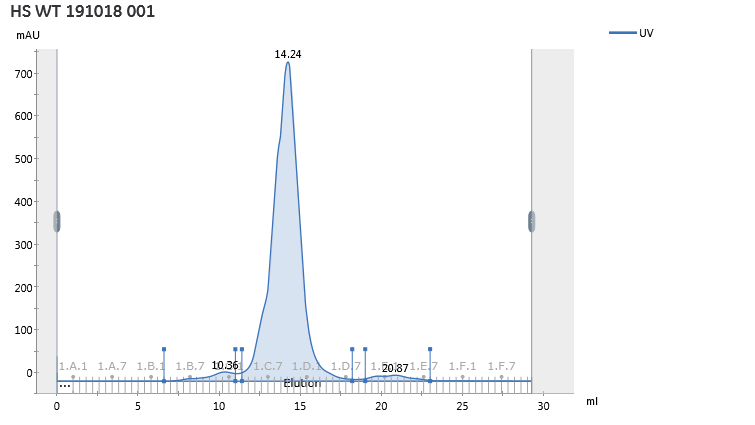
\includegraphics[width=\textwidth]{img/sec_wt}
        \caption{SEC graph of wildtype}
        \label{fig:sec_wt}
    \end{subfigure}
    ~
    \begin{subfigure}{0.45\textwidth}
        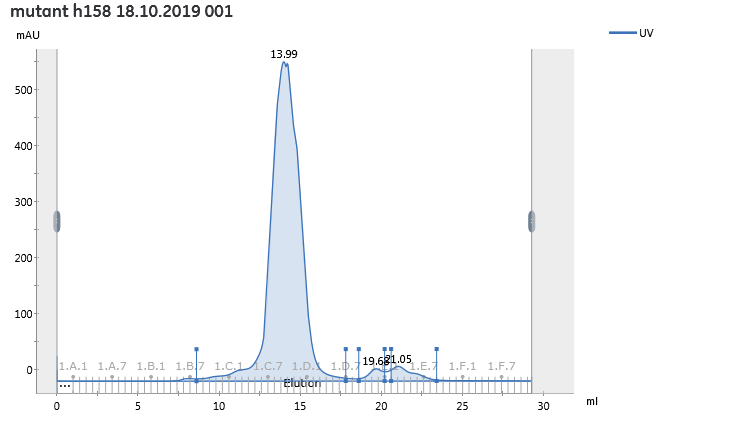
\includegraphics[width=\textwidth]{img/sec_mut}
        \caption{SEC graph of mutant}
        \label{fig:sec_mut}
    \end{subfigure}

    \begin{subfigure}{0.45\textwidth}
        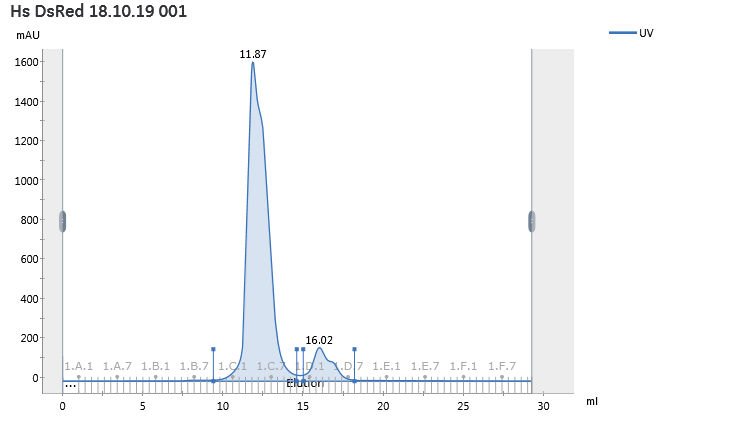
\includegraphics[width=\textwidth]{img/sec_dsred}
        \caption{SEC graph of dsRed}
        \label{fig:sec_dsred}
    \end{subfigure}
    \caption{SEC graphs of three SOO variants}
    \label{fig:sec}
\end{figure}

\section{Protein concentration determination}

Figure \ref{fig:hs_concentration} shows the absorption of the three protein
samples at various wavelengths. The absorption of use to us is the one at
\SI{561}{\nm} which is the absorbance of the two hemes within SOO.

In a first step, the absorption difference at \SI{561}{\nm} between the
oxidated and reduced forms was calculated. In order to compensate the fact that
the baseline of the reduced form was lower, the average absorption difference
in the range of \SIrange{580}{600}{\nm} was calculated, and added to the
previously calculated absorption difference at \SI{561}{\nm}.

Finally, using the path length of the cuvette of \SI{1}{\cm}, the provided
extinction coefficient of \SI{46.36}{\per\milli\Molar\per\cm} and the dilution
factor of \SI{375} the protein concentration was calculated using Beer's law.
These metrics including the final concentration are shown in table
\ref{tbl:hs_concentration}.

\begin{figure}
	\centering
	\includegraphics[width=0.8\textwidth]{img/hs_concentration.png}
	\caption{Absorption of HS for concentration determination}
	\label{fig:hs_concentration}
\end{figure}

\begin{table}
	\centering
	\begin{tabu}{lllll}
		\toprule
		Protein & $\Delta_{\text{Absorption at \SI{561}{\nm}}}$ & Baseline & $\Delta_{\text{Absorption at \SI{561}{\nm} corr}}$ & Concentration [\si{\milli\Molar}] \\
		\midrule
		Wildtype & 0.042 & 0.004 & 0.046 & 0.372 \\
		Mutant & 0.043 & 0.006 & 0.049 & 0.396 \\
		dsRed & 0.068 & 0.013 & 0.081 & 0.655 \\
		\bottomrule
	\end{tabu}
	\caption{Concentration of purified HS}
	\label{tbl:hs_concentration}
\end{table}

\section{SDS PAGE}

The results of the SDS page gels are shown in figure \ref{fig:sds}.

\begin{figure}[h!]
    \centering
    \begin{subfigure}{0.7\textwidth}
        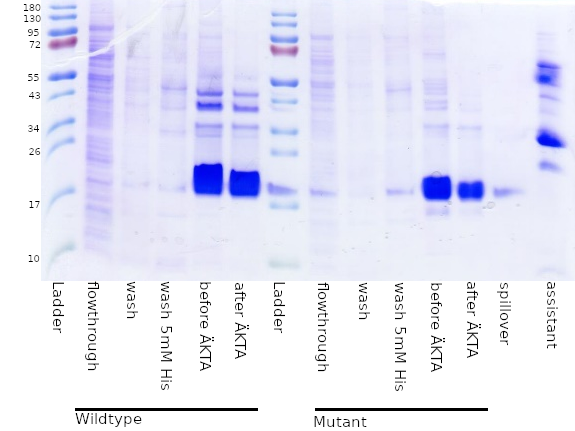
\includegraphics[width=\textwidth]{img/sds_wt_mut}
        \caption{SDS PAGE gel of wildtype and mutant}
        \label{fig:sds_wt_mut}
    \end{subfigure}

    \begin{subfigure}{0.7\textwidth}
        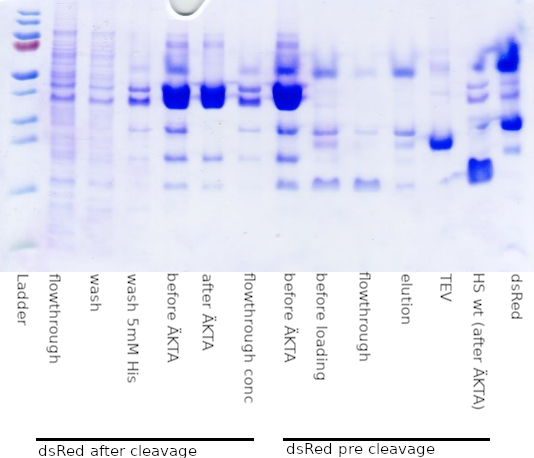
\includegraphics[width=\textwidth]{img/sds_dsred_tev_cleavage.png}
        \caption{SDS PAGE gel of dsRed including cleaved dsRed}
        \label{fig:sds_dsred_cleaved}
    \end{subfigure}
    \caption{SDS gels of three protein variants}
    \label{fig:sds}
\end{figure}

\section{Fluorescence measurements}

The results of the fluorescence measurements for tracking losses during
purification are shown in figure \ref{fig:purification_fluorescence}.
Fluorescence measurements were scaled to the volume the sample had at the time
of the aliquot being stored. This allowed using the so-adjusted fluorescence
value as an indicator of the amount of protein - rather than the concentration
of protein - which were present in the sample at the given stage.

\begin{figure}
	\centering
	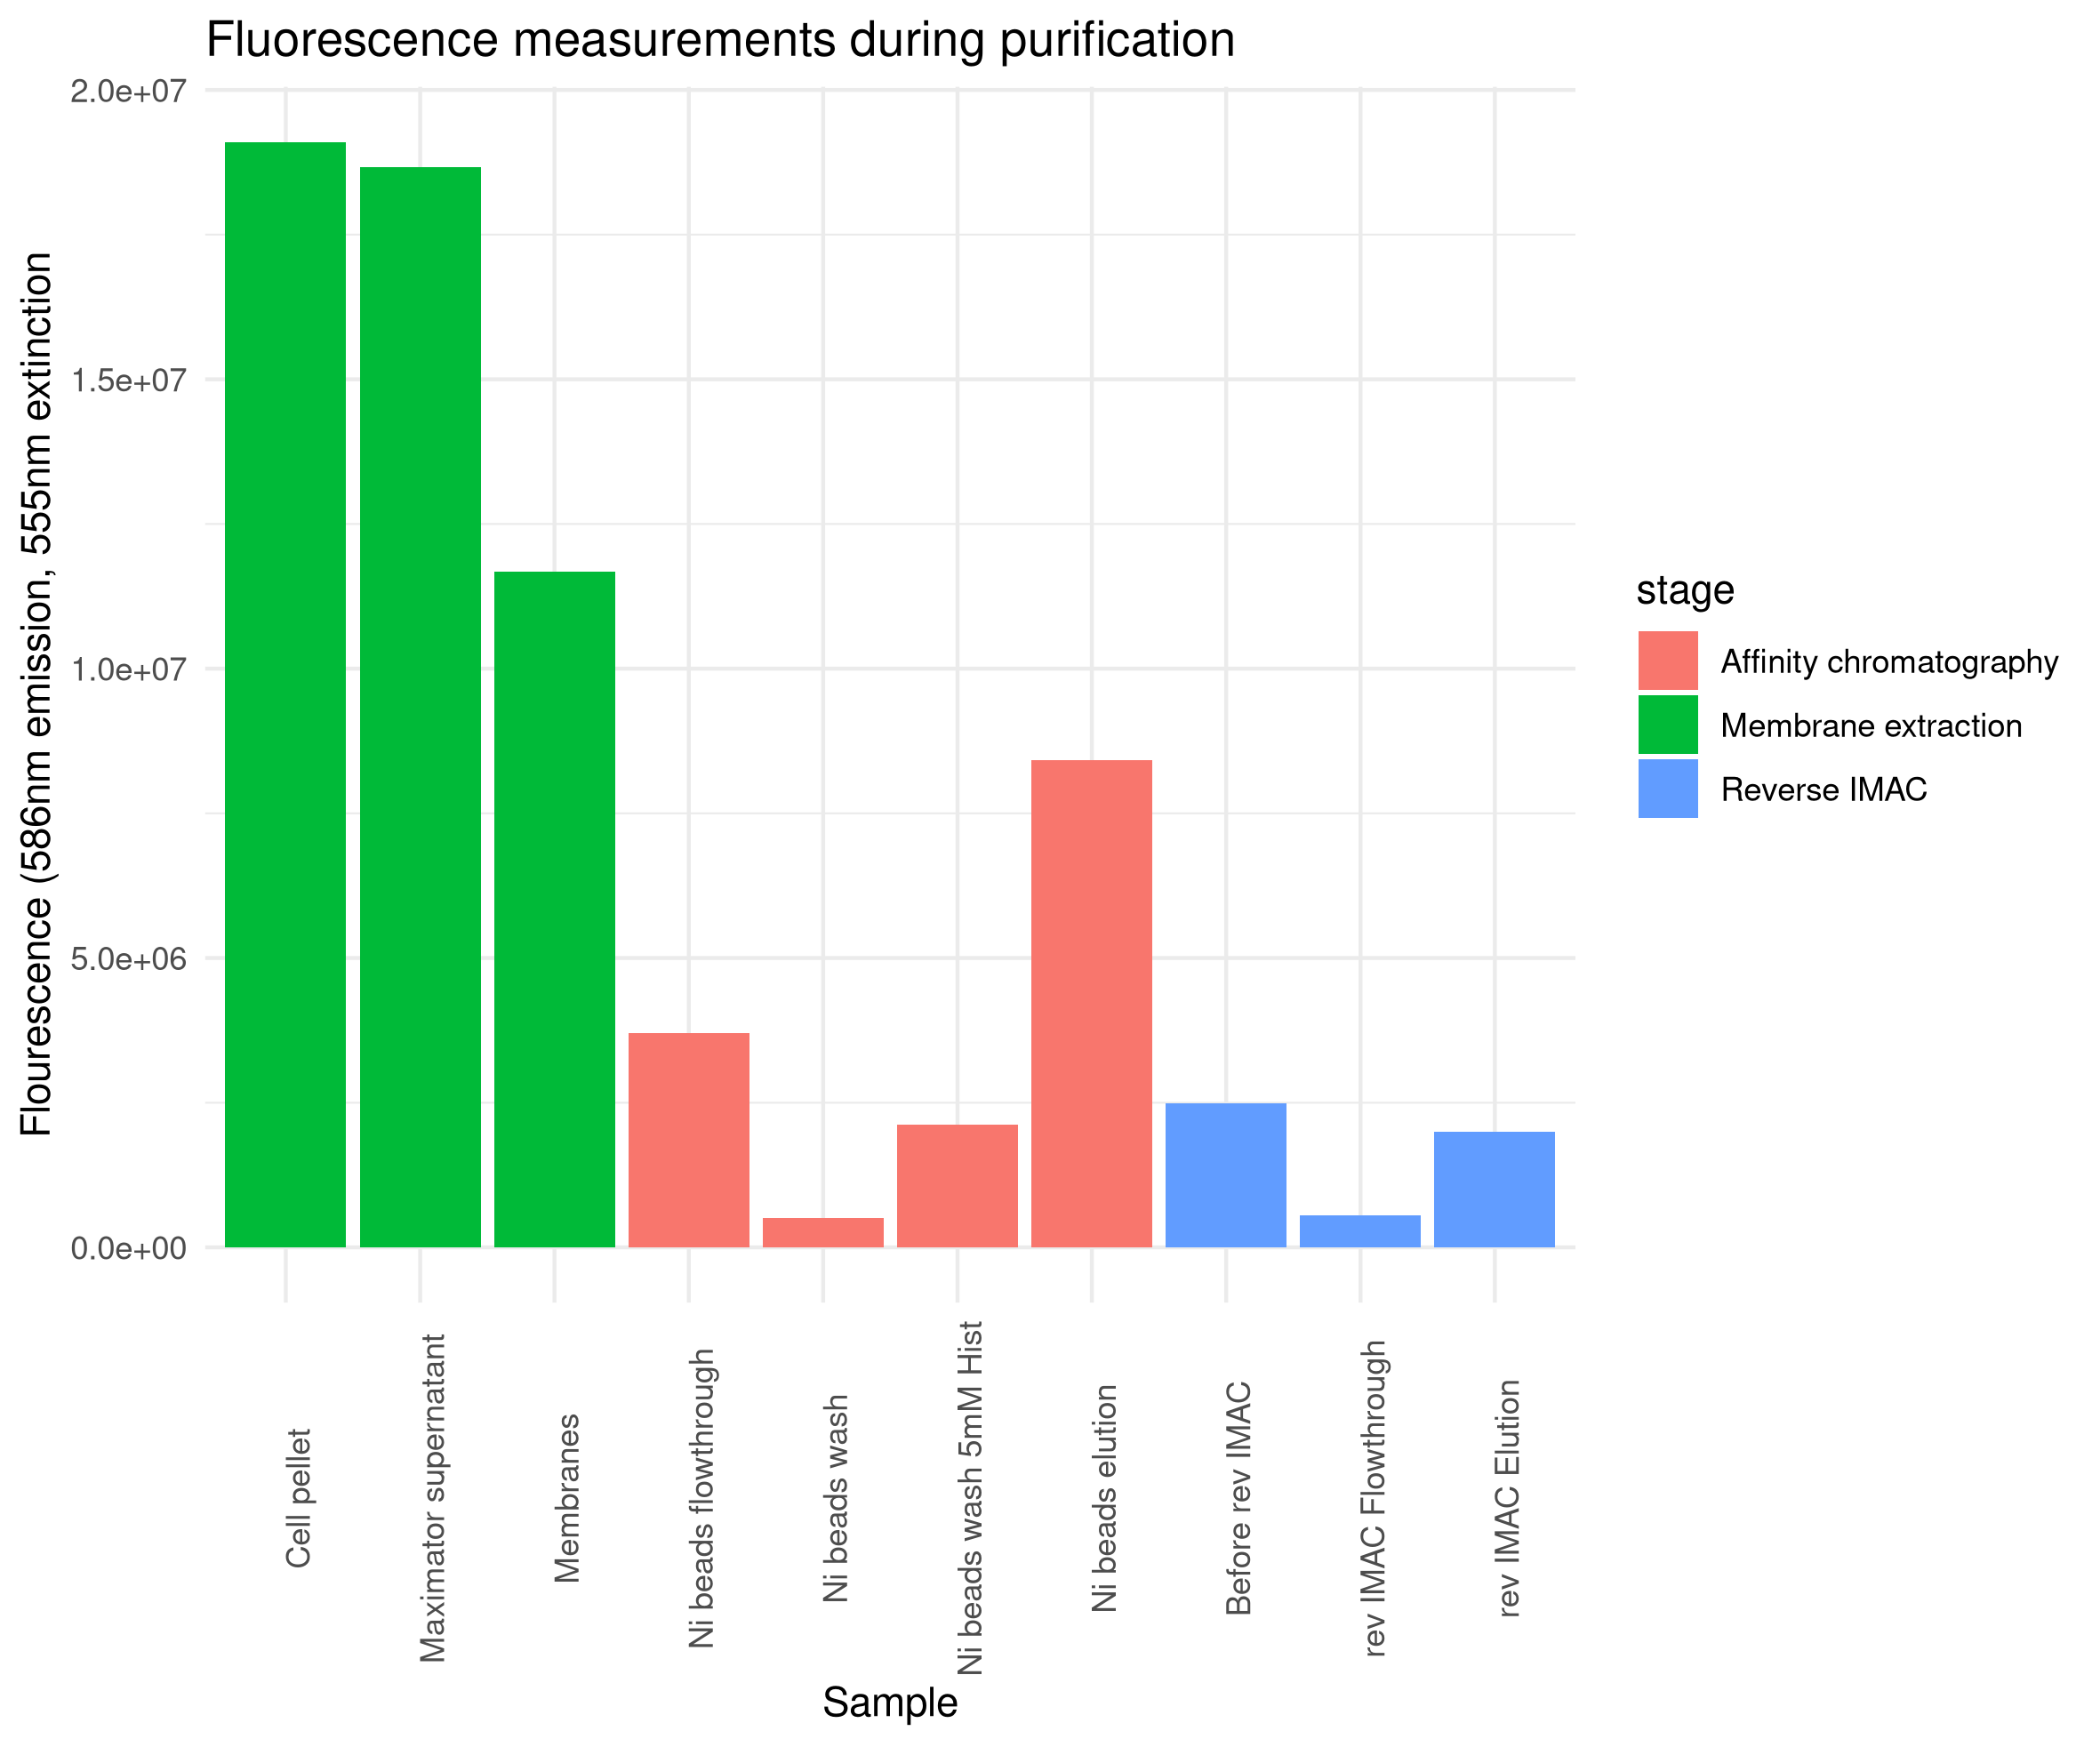
\includegraphics[width=0.8\textwidth]{img/purification_fluorescence.png}
	\caption{Fluorescence measurements to track purification losses}
	\label{fig:purification_fluorescence}
\end{figure}

\section{Relative enzyme reduction}

\subsection{Quinone}

The absorption measurements of the wildtype, mutant and control to follow the
reduction of HS are shown in figure \ref{fig:reduction_quinol}.

To determine the relative reduction of HS by quinol, three absorption values
were considered. The average absorption value between \SIrange{0.8}{0.9}{\min}
was used as a baseline, which was subtracted from the other two measurements.
The average absorption between \SIrange{2.5}{2.6}{\min} allowed following the
reduction of HS by quinol, while the average absorption between
\SIrange{3.9}{4}{\min} gave the absorption value where all HS had been reduced
by DTT. These three values, as well as the resulting relative reduction of HS
by quinol, are shown in table \ref{tbl:reduction_quinol}.

\begin{figure}
	\centering
	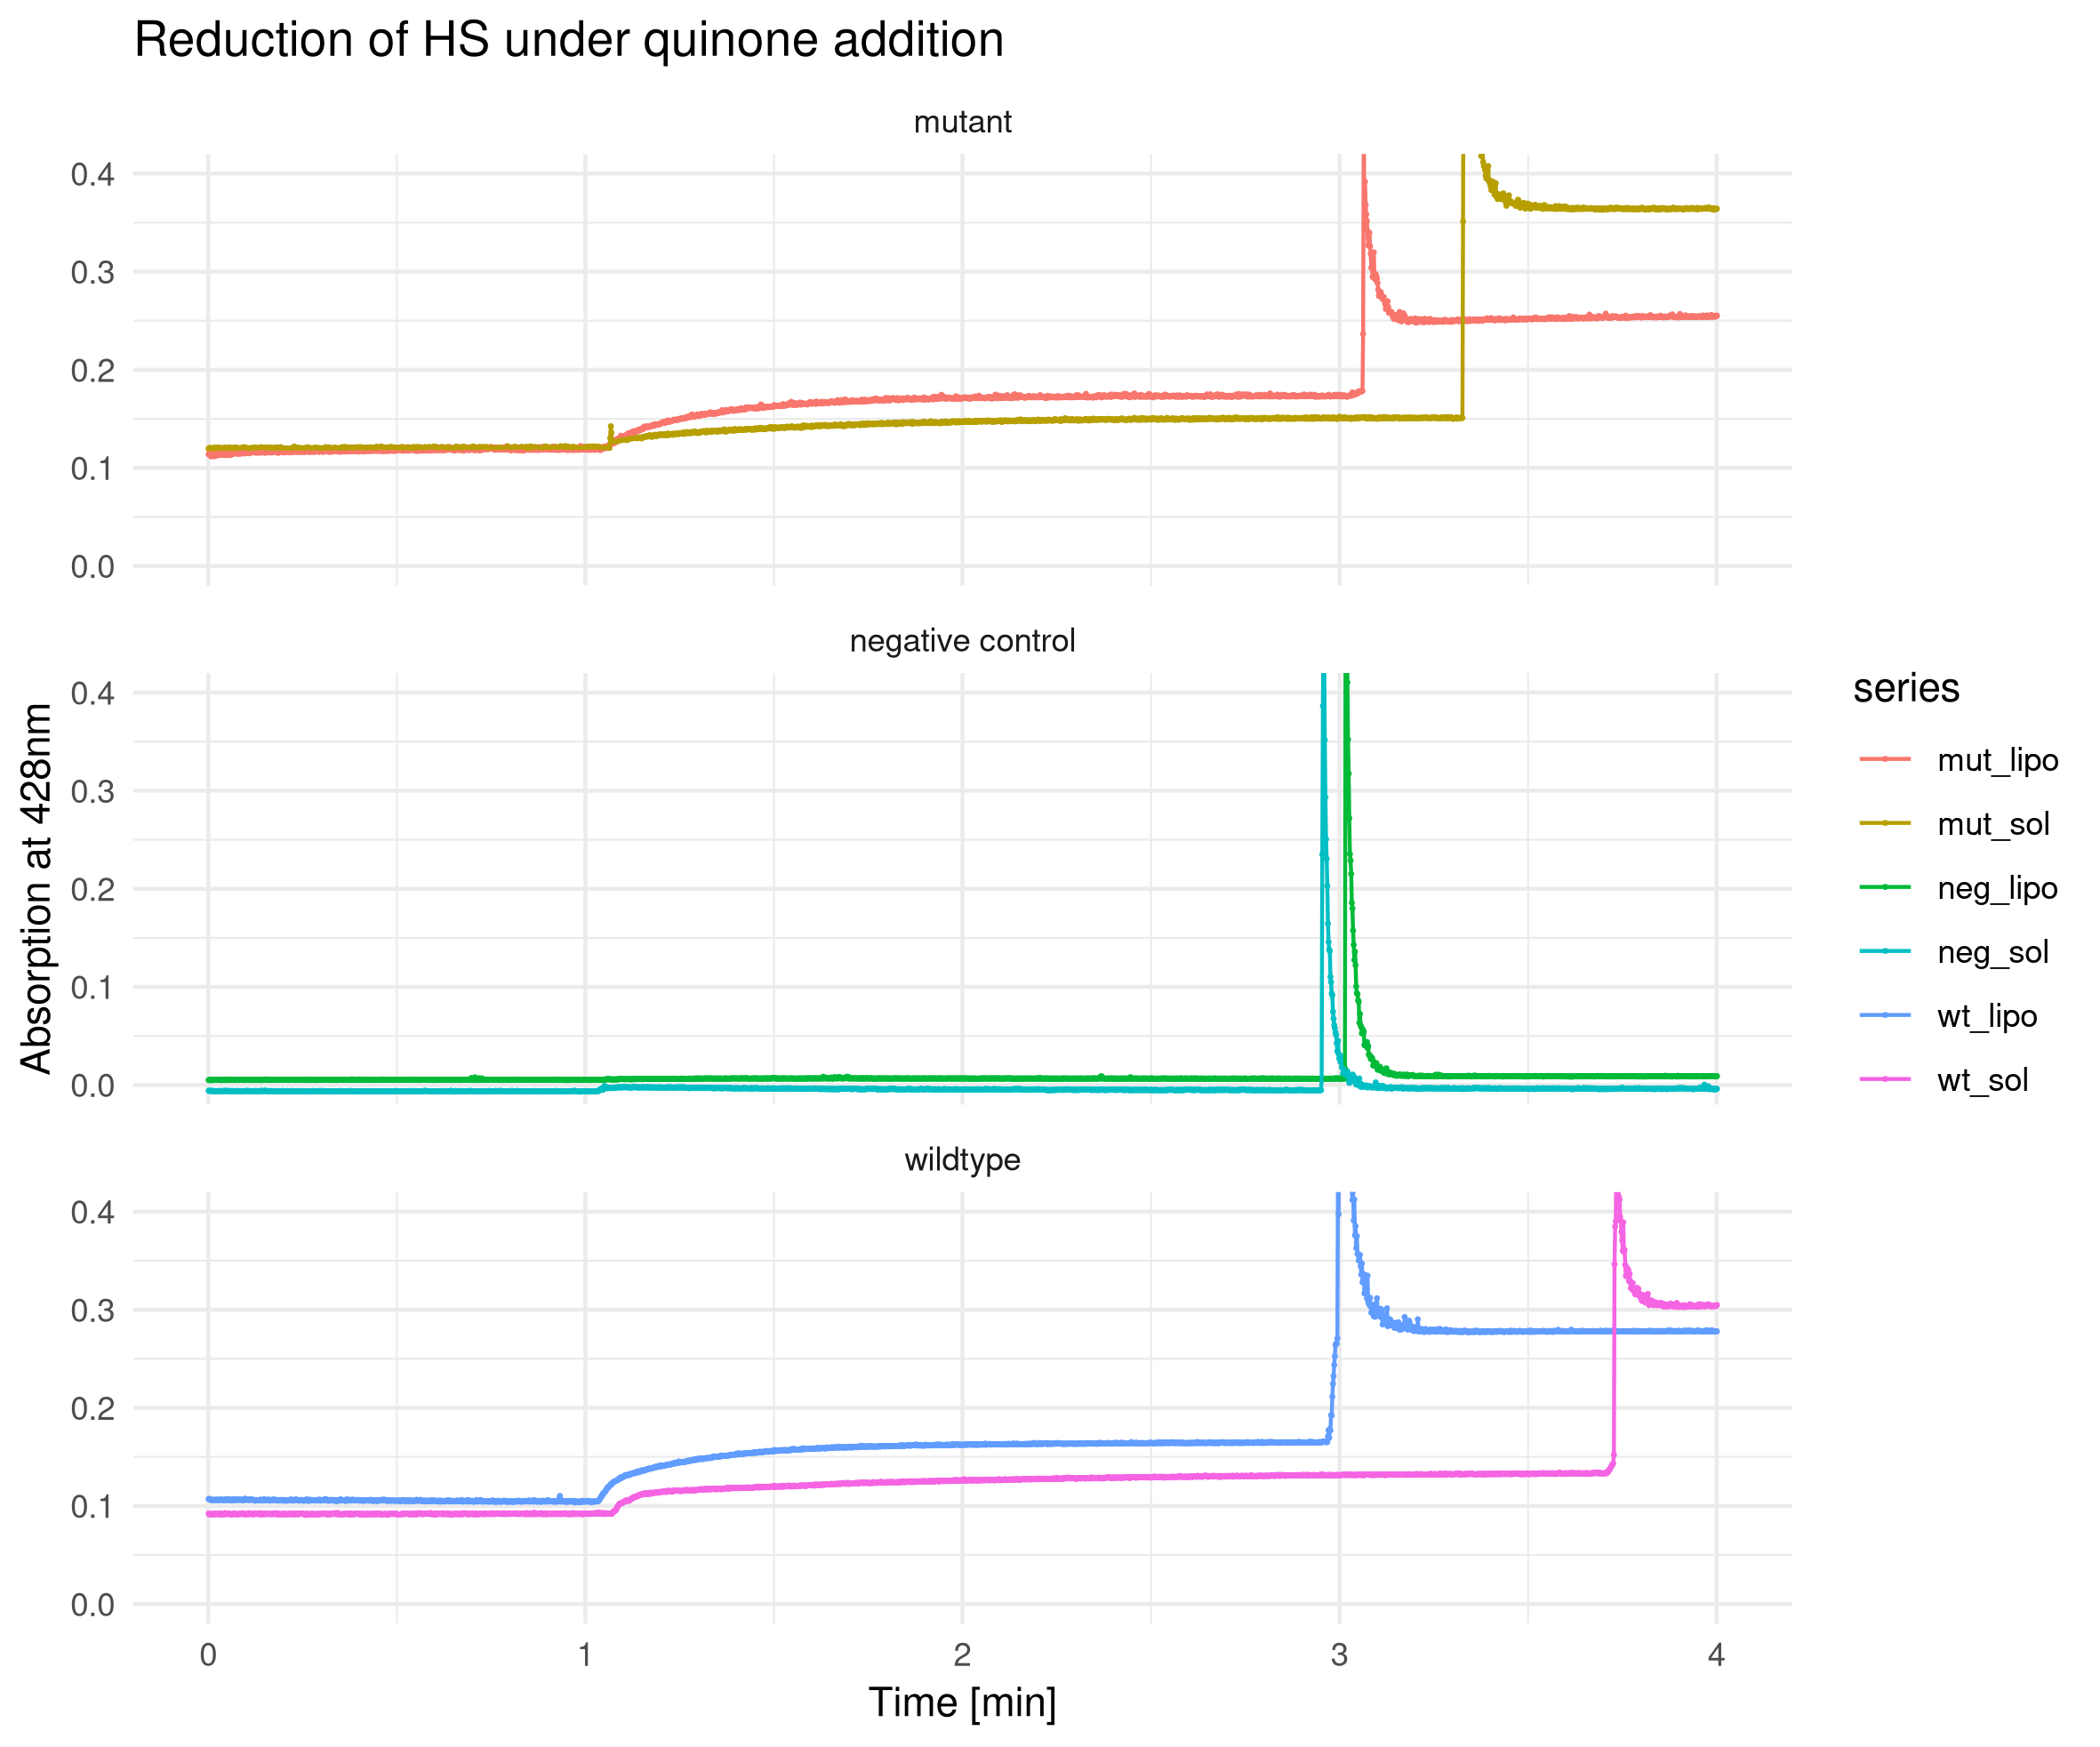
\includegraphics[width=0.8\textwidth]{img/reduction_quinol.png}
	\caption{Absorbance of HS to track reduction due to quinol}
	\label{fig:reduction_quinol}
\end{figure}


\begin{table}
	\centering
	\begin{tabu}{llllll}
		\toprule
		Protein & State & Baseline & Absorption Quinol & Absorption \SI{100}{\percent} & Rel reduction \\
		\midrule
		Wildtype & Liposomes & 0.105 & 0.164 & 0.278 & \SI{34}{\percent} \\
		Wildtype & Solubilized & 0.092 & 0.130 & 0.304 & \SI{18}{\percent} \\
		Mutant & Liposomes & 0.119 & 0.173 & 0.254 & \SI{40}{\percent} \\
		Mutant & Solubilized & 0.121 & 0.150 & 0.364 & \SI{12}{\percent} \\
		\bottomrule
	\end{tabu}
	\caption{Relative reduction of HS by quinol addition}
	\label{tbl:reduction_quinol}
\end{table}

\subsection{Superoxide}

The corresponding graphs and tables for the reduction of HS in presence of
superoxide are shown in figure \ref{fig:reduction_superox} and table
\ref{tbl:reduction_superox}.

\begin{figure}
	\centering
	\includegraphics[width=0.9\textwidth]{img/reduction_superox.png}
	\caption{Absorbance of HS to track reduction due to superoxide}
	\label{fig:reduction_superox}
\end{figure}

\begin{table}
	\centering
	\begin{tabu}{lllllll}
		\toprule
		Protein & State & SOD & Baseline & Abs Superox & Abs \SI{100}{\percent} & Rel reduction \\
		\midrule
		Mutant   & Liposomes   & No   &          0.0854    &            0.103               &   0.218         &  \SI{14}{\percent}   \\
		Mutant   & Liposomes   & Yes  &            0.0815  &              0.0828            &     0.202       &  \SI{01}{\percent}  \\
		Mutant   & Solubilized & No   &          0.0650    &            0.118               &   0.251         &  \SI{28}{\percent}   \\
		Mutant   & Solubilized & Yes  &            0.0862  &              0.0892            &     0.276       &  \SI{02}{\percent}  \\
		Wildtype & Liposomes   & No   &          0.103     &            0.126               &   0.279         &  \SI{13}{\percent}  \\
		Wildtype & Liposomes   & Yes  &            0.0820  &              0.0846            &     0.272       &  \SI{1 }{\percent} \\
		Wildtype & Solubilized & No   &          0.0874    &            0.143               &   0.277         &  \SI{29}{\percent}  \\
		Wildtype & Solubilized & Yes  &            0.0980  &              0.0985            &     0.280       &  \SI{0 }{\percent} \\
		\bottomrule
	\end{tabu}
	\caption{Relative reduction of HS by superox addition}
	\label{tbl:reduction_superox}
\end{table}

\subsection{Relative reduction}

The relative reductions by both, superoxide and quinol, are shown in figure
\ref{fig:reduction_relative}.

\begin{figure}
    \centering
    \begin{subfigure}{0.45\textwidth}
	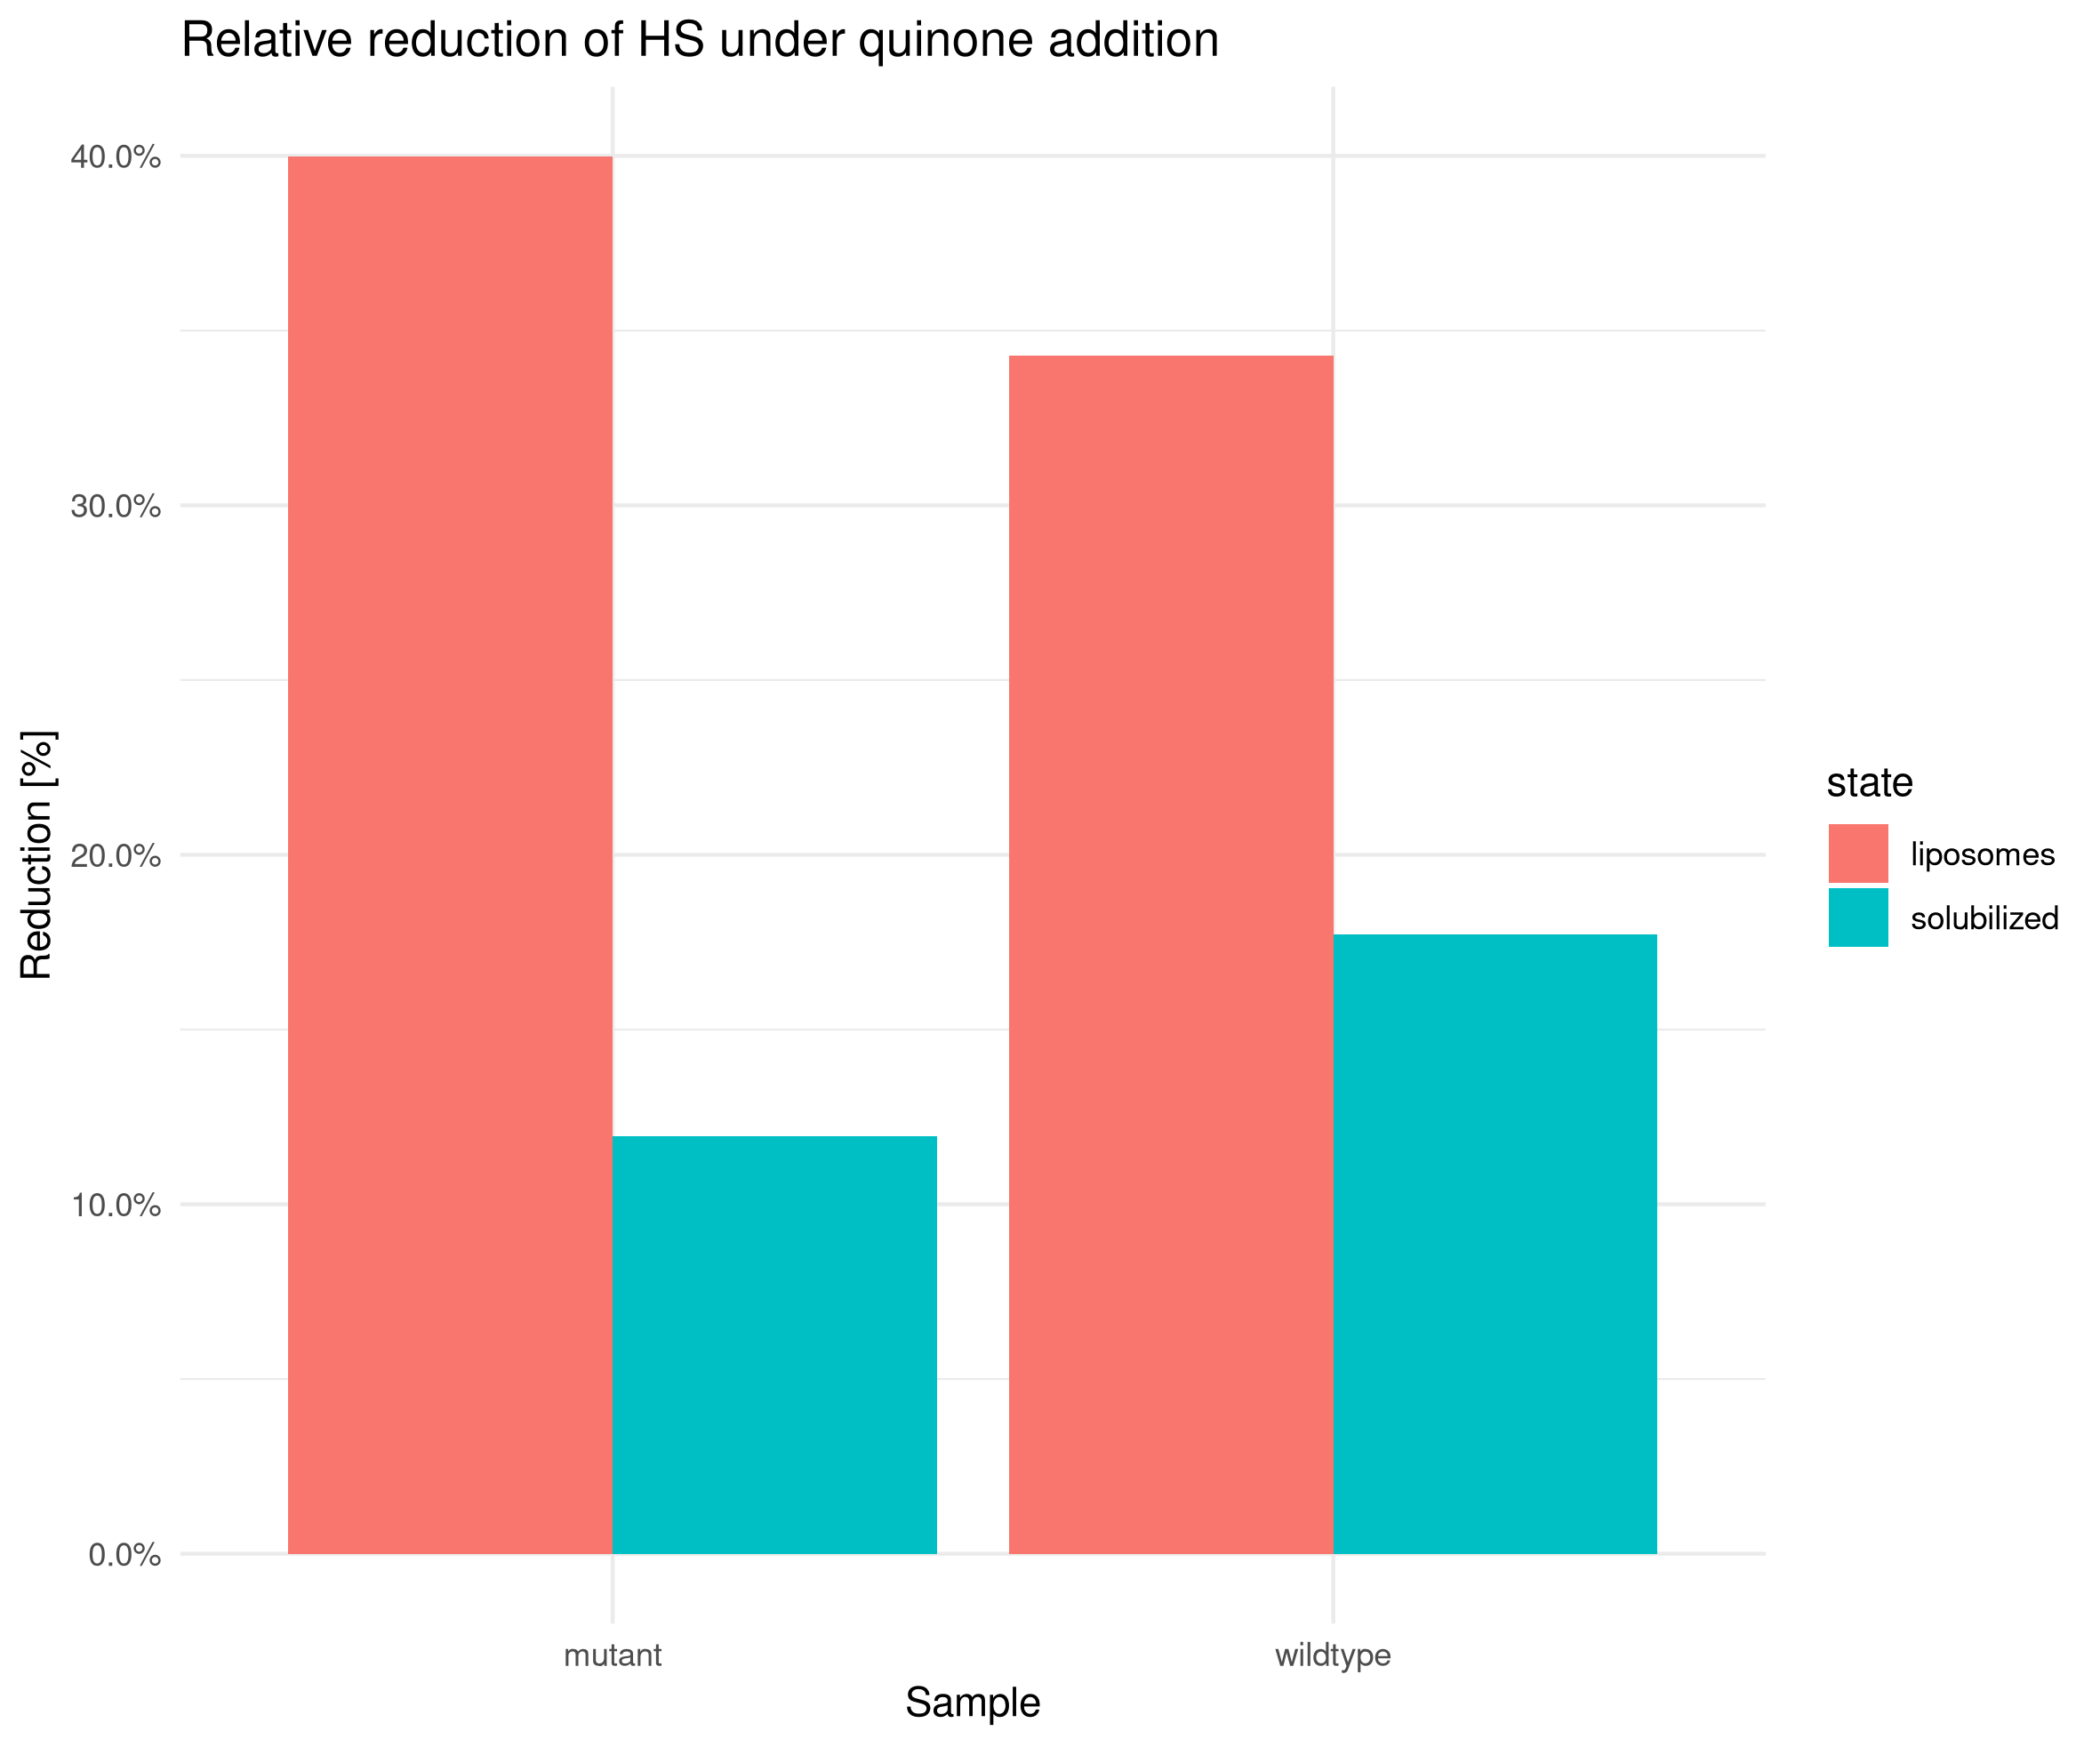
\includegraphics[width=\textwidth]{img/reduction_quinol_relative.png}
	\caption{Relative reduction of HS by quinol}
	\label{fig:reduction_quinol_relative}
    \end{subfigure}
    ~
    \begin{subfigure}{0.45\textwidth}
	\centering
	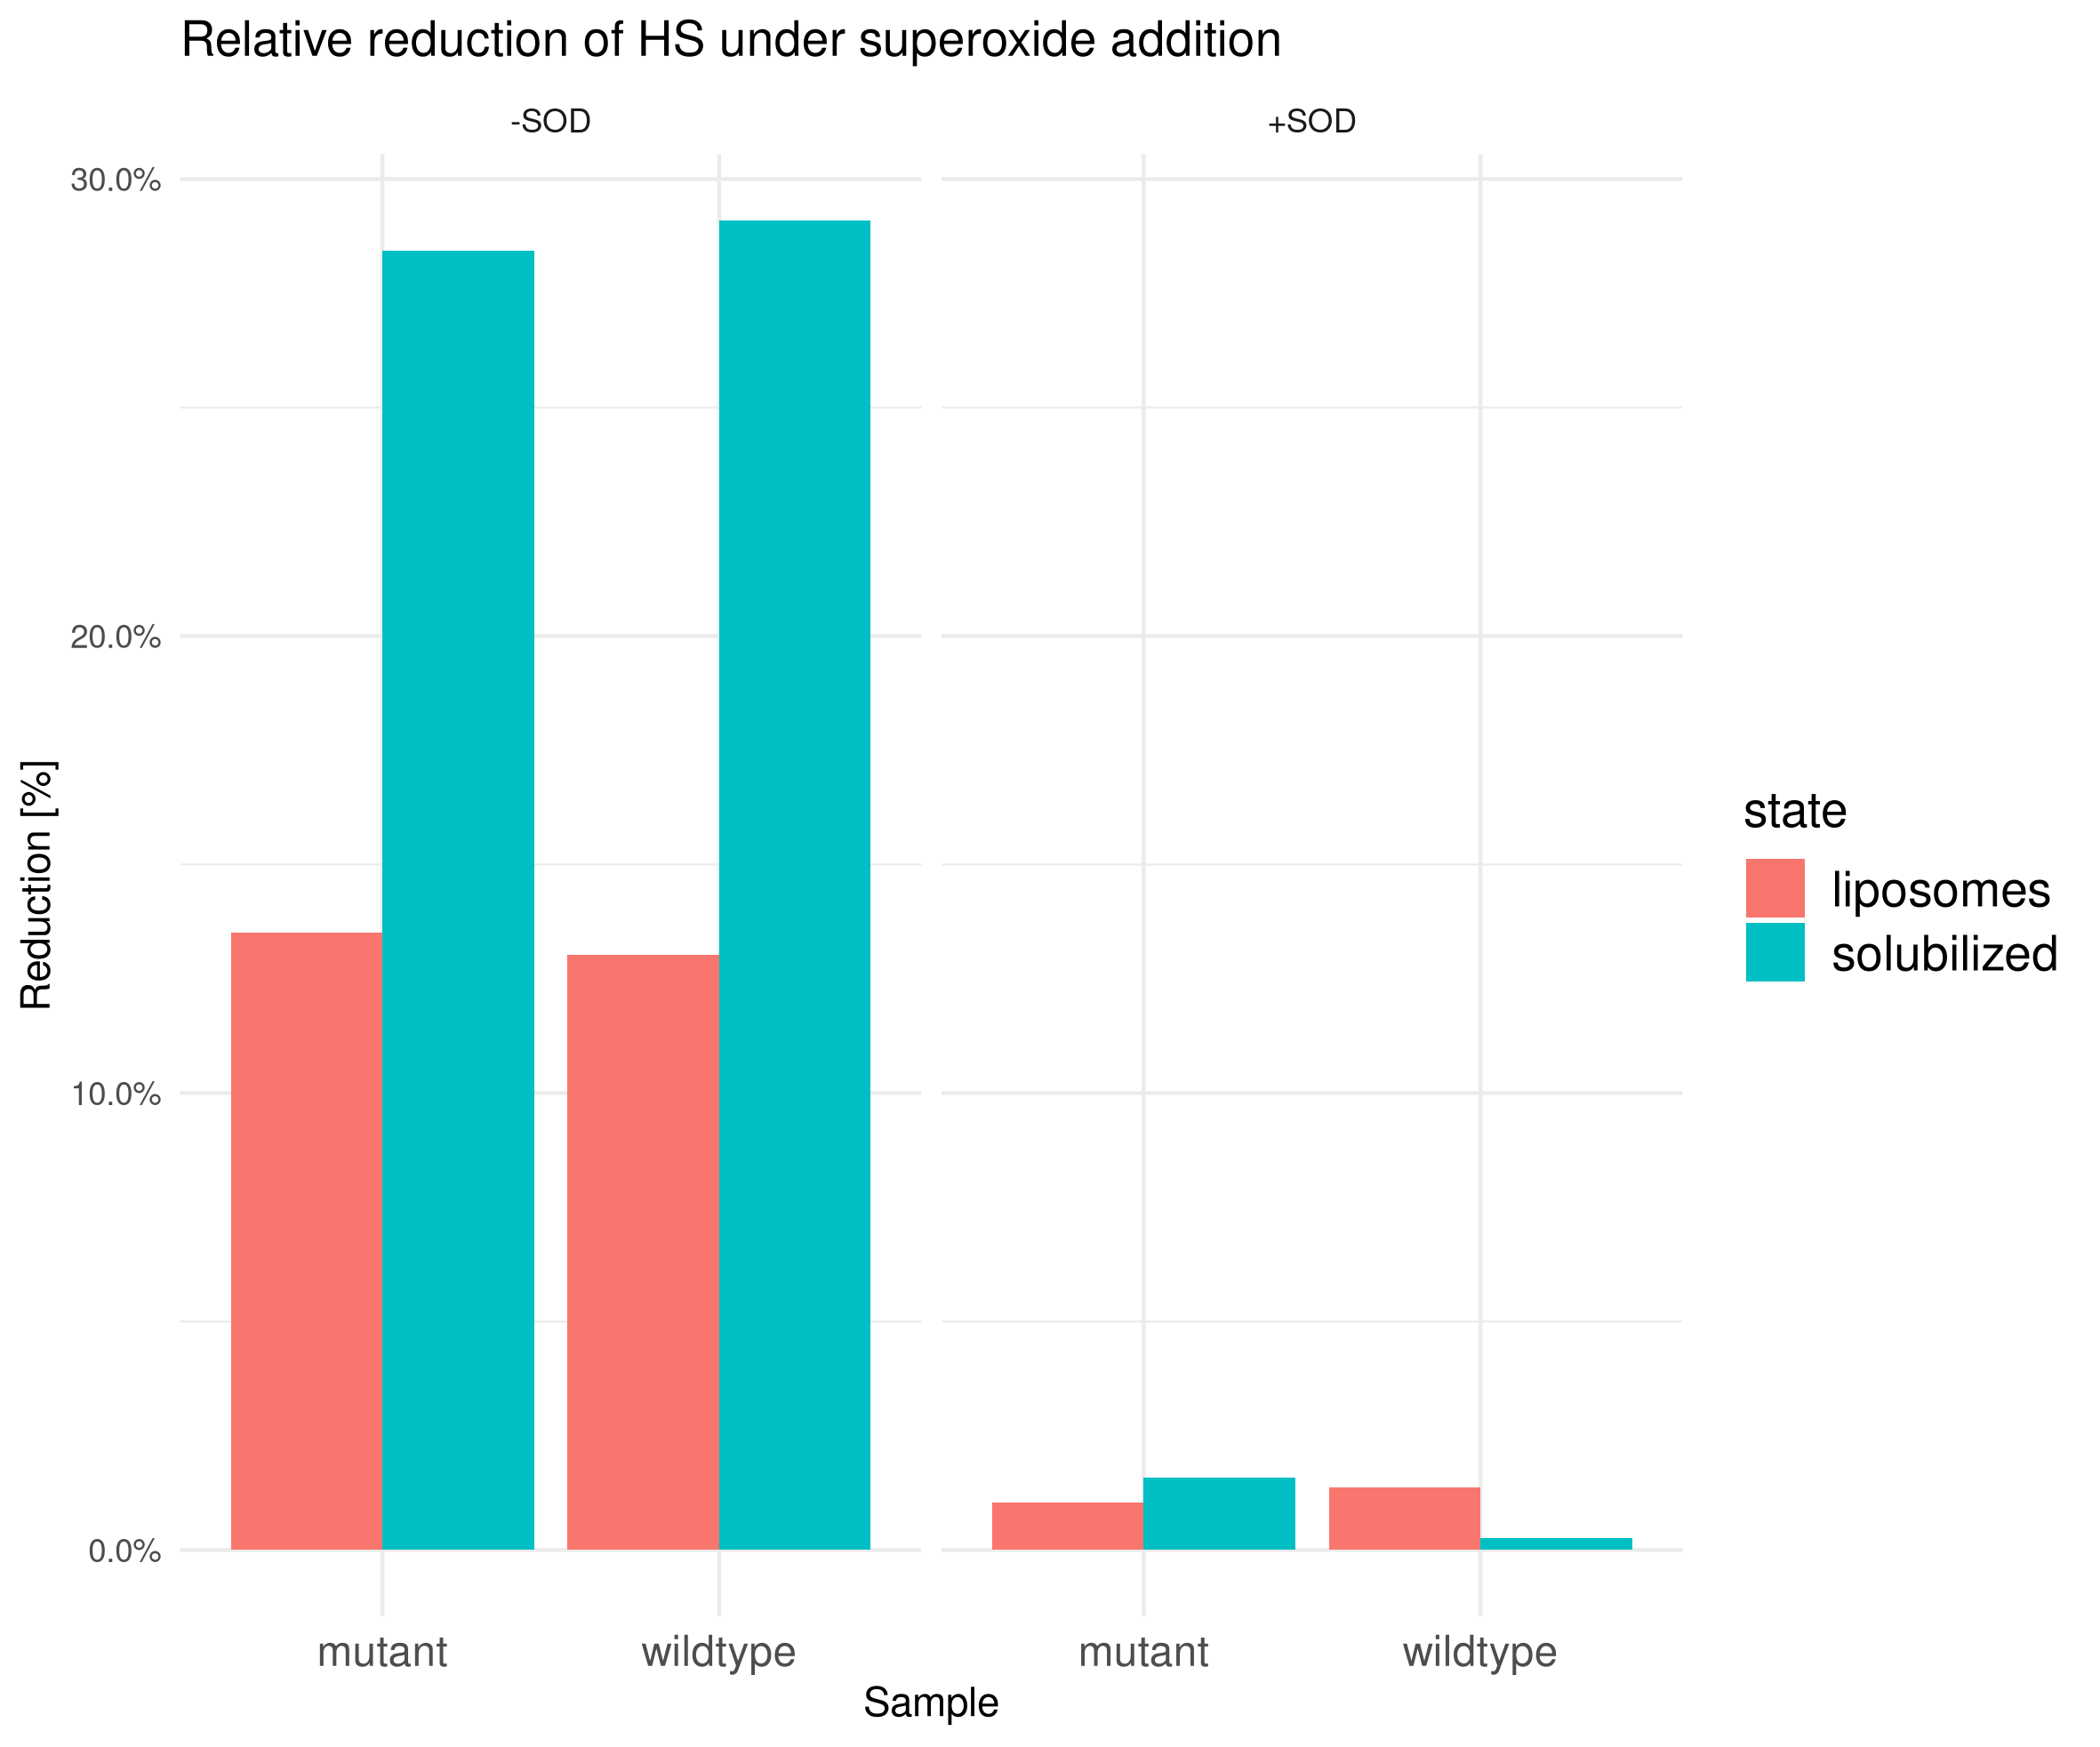
\includegraphics[width=\textwidth]{img/reduction_superox_relative.png}
	\caption{Relative reduction of HS by superox}
	\label{fig:reduction_superox_relative}
    \end{subfigure}
    \caption{Relative reduction of HS by quinol and superoxide}
    \label{fig:reduction_relative}
\end{figure}

\section{Fluorescence measurements before and after cleavage}

The results of the various fluorescence measurements of cleaved and uncleaved
HS-dsRed including the quenching with copper are shown in figure
\ref{fig:dsred_cleavage_fluorescence}.

\begin{figure}
	\centering
	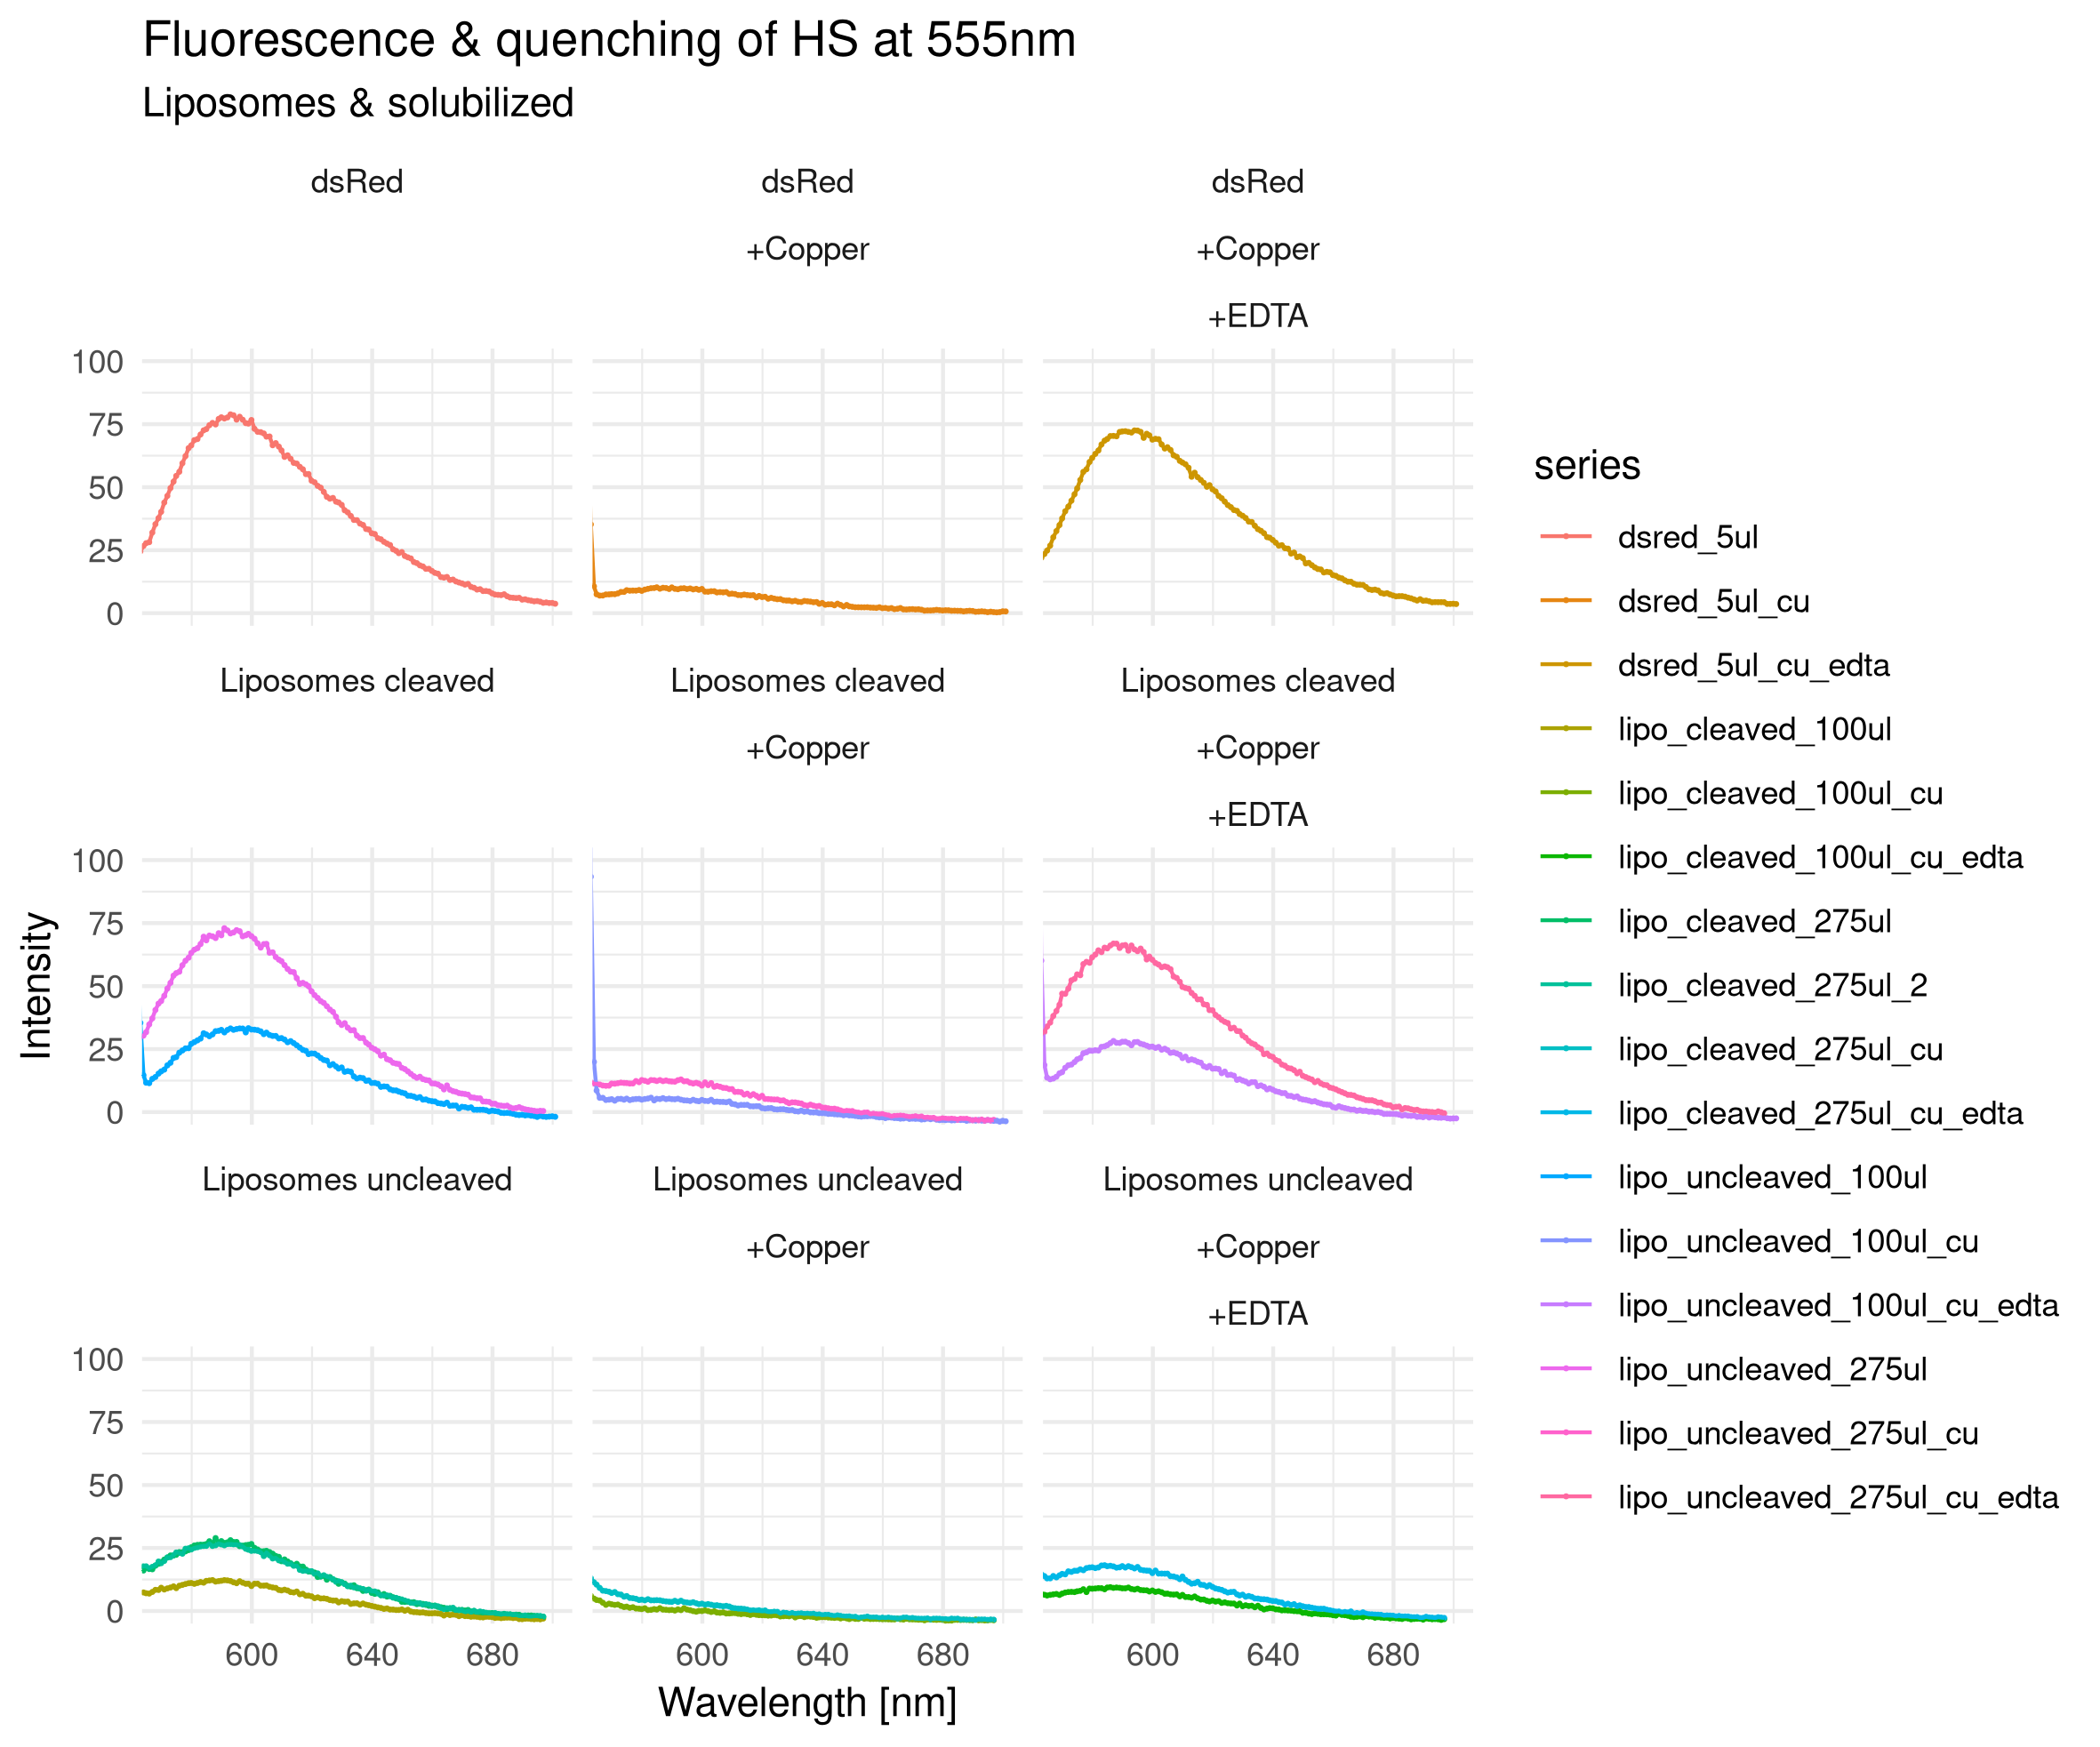
\includegraphics[width=\textwidth]{img/dsred_cleavage_fluorescence.png}
	\caption{Fluorescence and quenching thereof of cleaved and uncleaved dsRed}
	\label{fig:dsred_cleavage_fluorescence}
\end{figure}

\section{Activity measurement}

\subsection{Determining sufficient HS concentrations}

Figures \ref{fig:activity_mut_hs} and \ref{fig:activity_wt_hs} show the
absorption graphs which were used to determine HS concentrations which were
able to quench the reduction of the dye as well as SOD. For the mutant this
turned out to be a volume of \SI{9}{\ul} per cuvette, for the wild type a
volume of \SI{1}{\ul}.

\subsection{Determining $K_m$}

Figure \ref{fig:activity_quinone} shows the absorption graphs when quinone
concentration was gradually lowered. For each of the samples the slope after
enzyme addition was determined. As a baseline the slope of the SOD sample after
SOD addition was determined, as well as the average of all slopes after XO
addition.

This allowed calculating the relative oxidation of superoxide as follows. Let
$s_{\text{xo}}$ be the average slope after XO addition. Let $s_{\text{SOD}}$ be
the slope after SOD addition. Let $s_{\text{sample}}$ be the slope of one
sample after addition of enzyme. The relative oxidation of superoxide of that
one sample is then given as:

\[
	\text{oxidation}_{\text{Superoxide}} = 1 - \frac{s_{\text{sample}}}{s_{\text{XO}} - s_{\text{SOD}}}
\]

These relative oxidation values are shown in figure \ref{fig:activity_km}, as
well as in a LB plot in figure \ref{fig:activity_km_lb}. A linear regression
was performed on the values, which then allowed to calculate the following
$K_m$ values in table \ref{tbl:activity_km}.

\begin{table}
	\centering
	\begin{tabu}{lllll}
		\toprule
		Protein & LB slope $a$ & LB y-intercept $b$ & $v_{\text{max}} = b^{-1}$ & $K_m = v_{\text{max}} \cdot a$ \\
		\midrule
		Wildtype & 0.0065 & 1.1 & \SI{90.9}{\percent} & \SI{0.0059}{\micro\Molar} \\
		Mutant & 0.24 & 1.1 & \SI{90.9}{\percent} & \SI{0.218}{\micro\Molar} \\
		\bottomrule
	\end{tabu}
	\caption{Determination of $K_m$ for HS}
	\label{tbl:activity_km}
\end{table}


\begin{figure}
    \centering
    \begin{subfigure}{0.75\textwidth}
	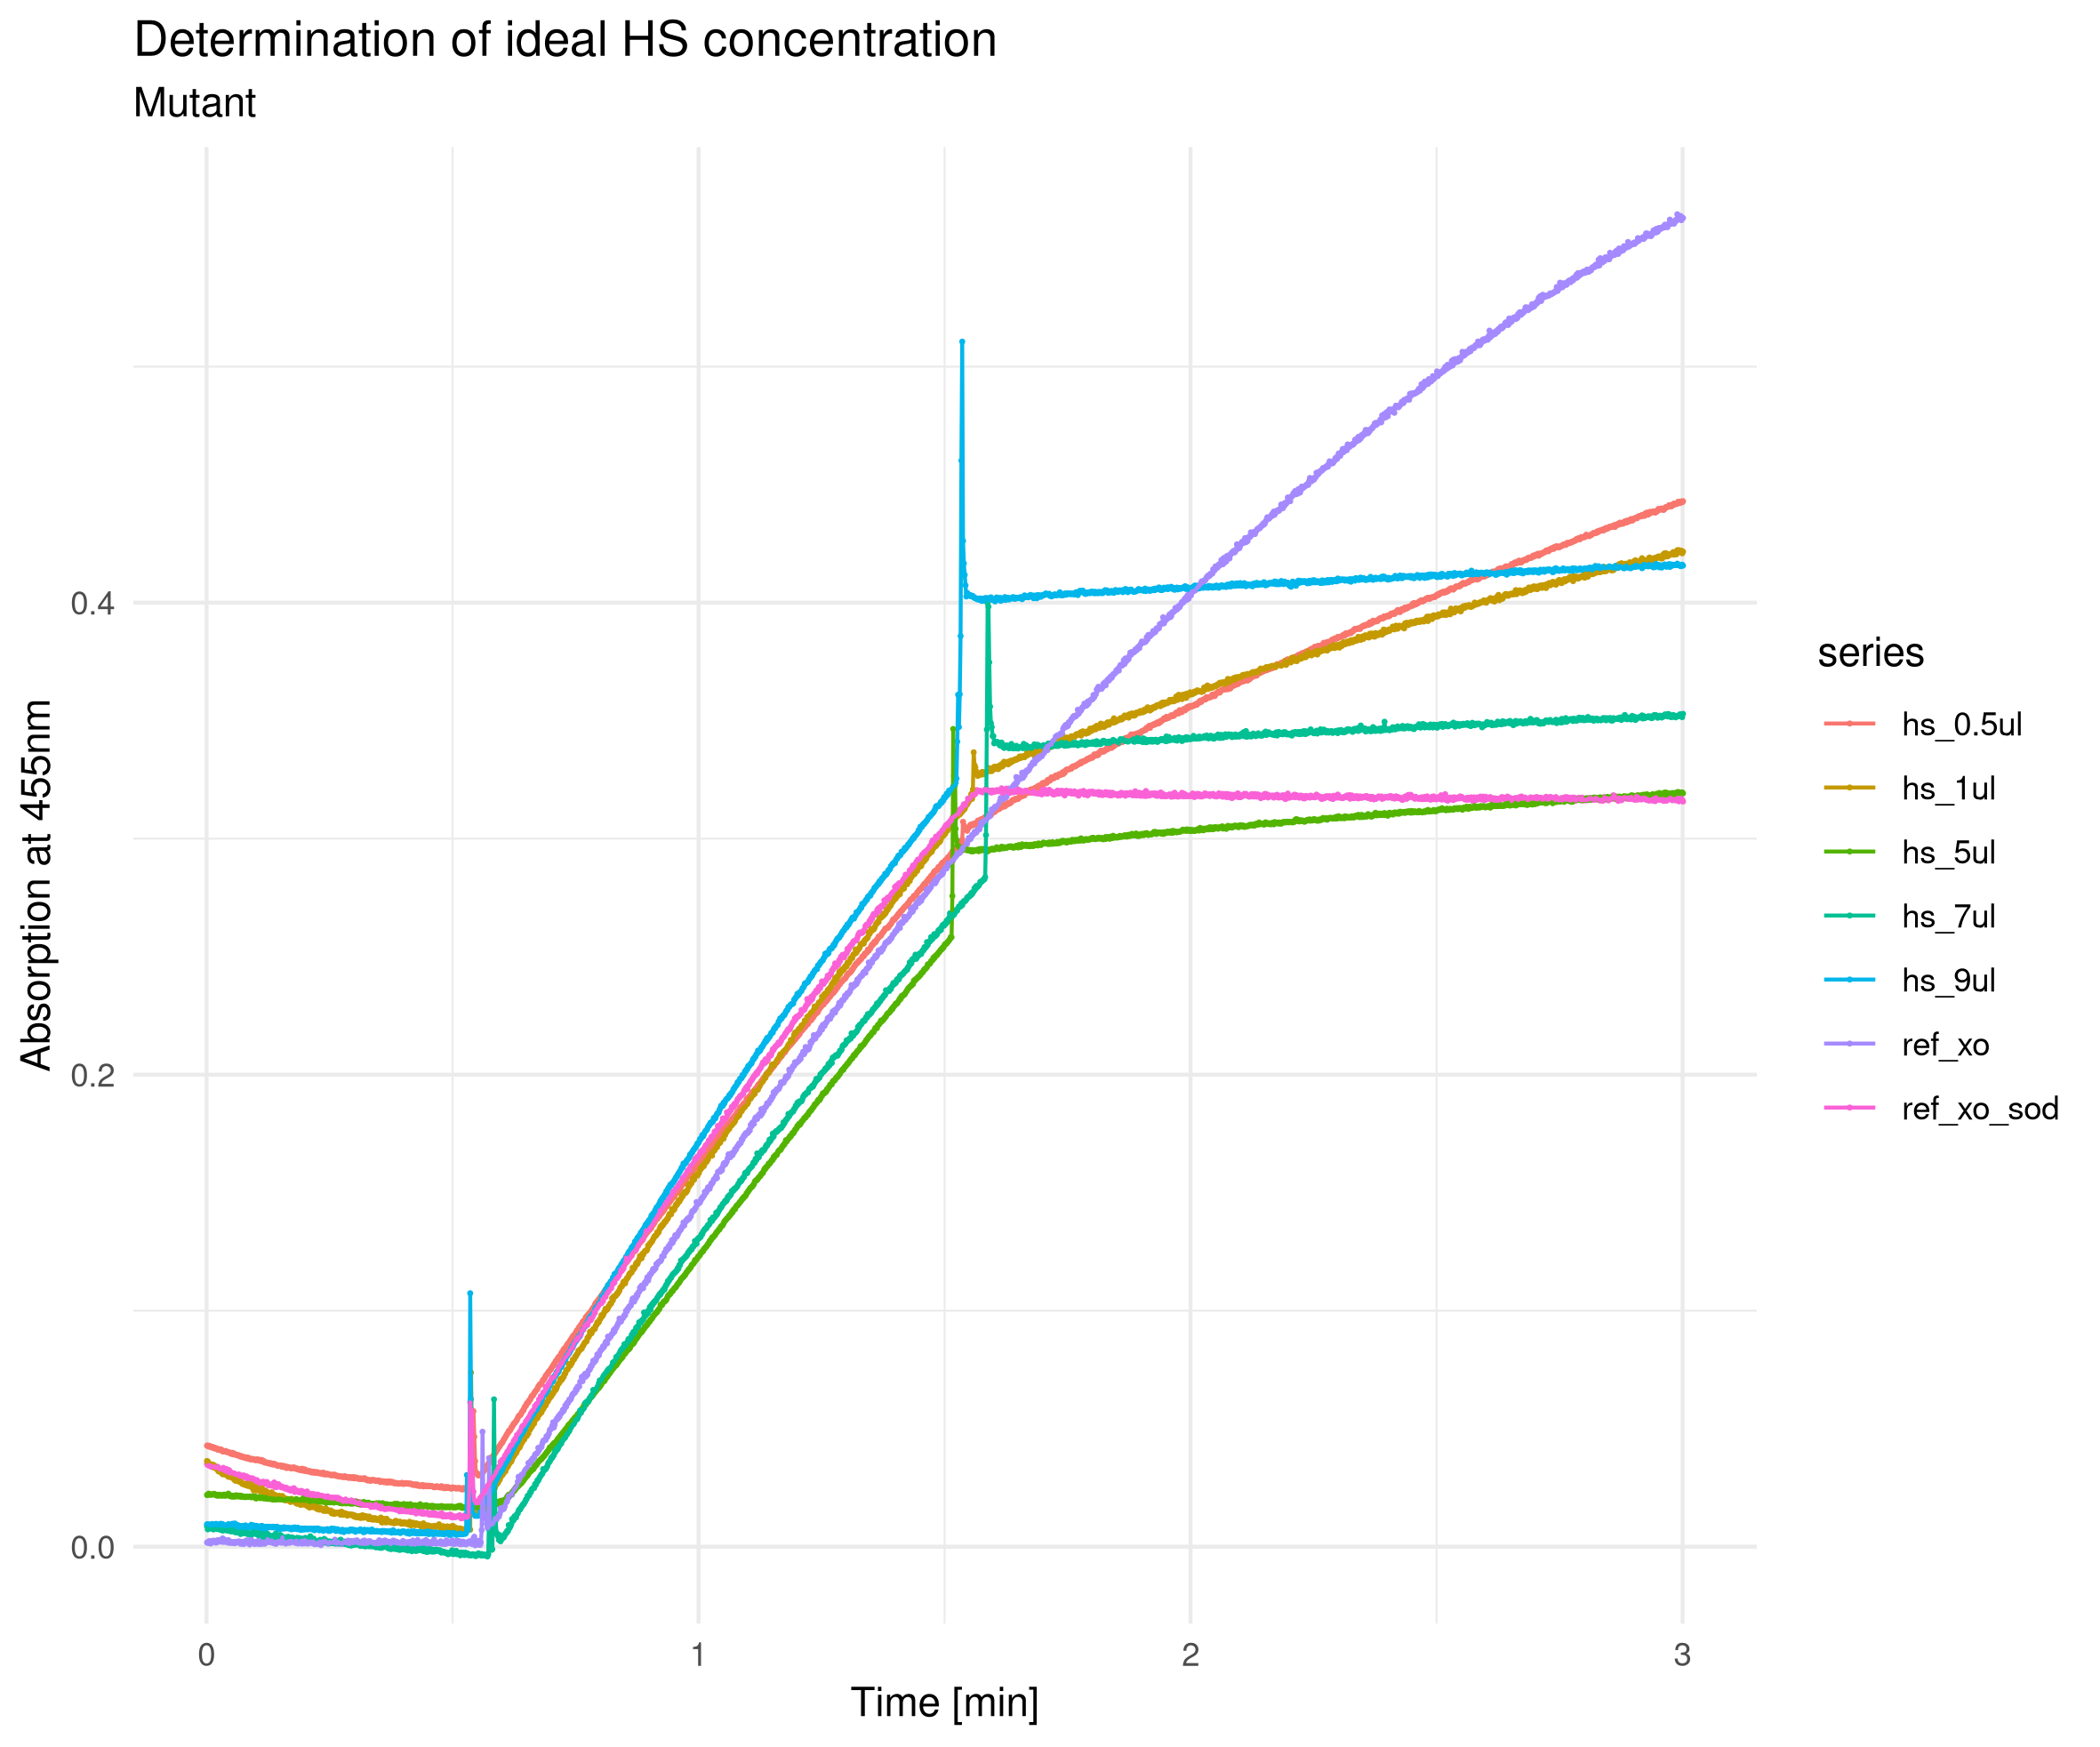
\includegraphics[width=\textwidth]{img/activity_mut_hs.png}
	\caption{HS mutant}
	\label{fig:activity_mut_hs}
    \end{subfigure}

    \begin{subfigure}{0.75\textwidth}
	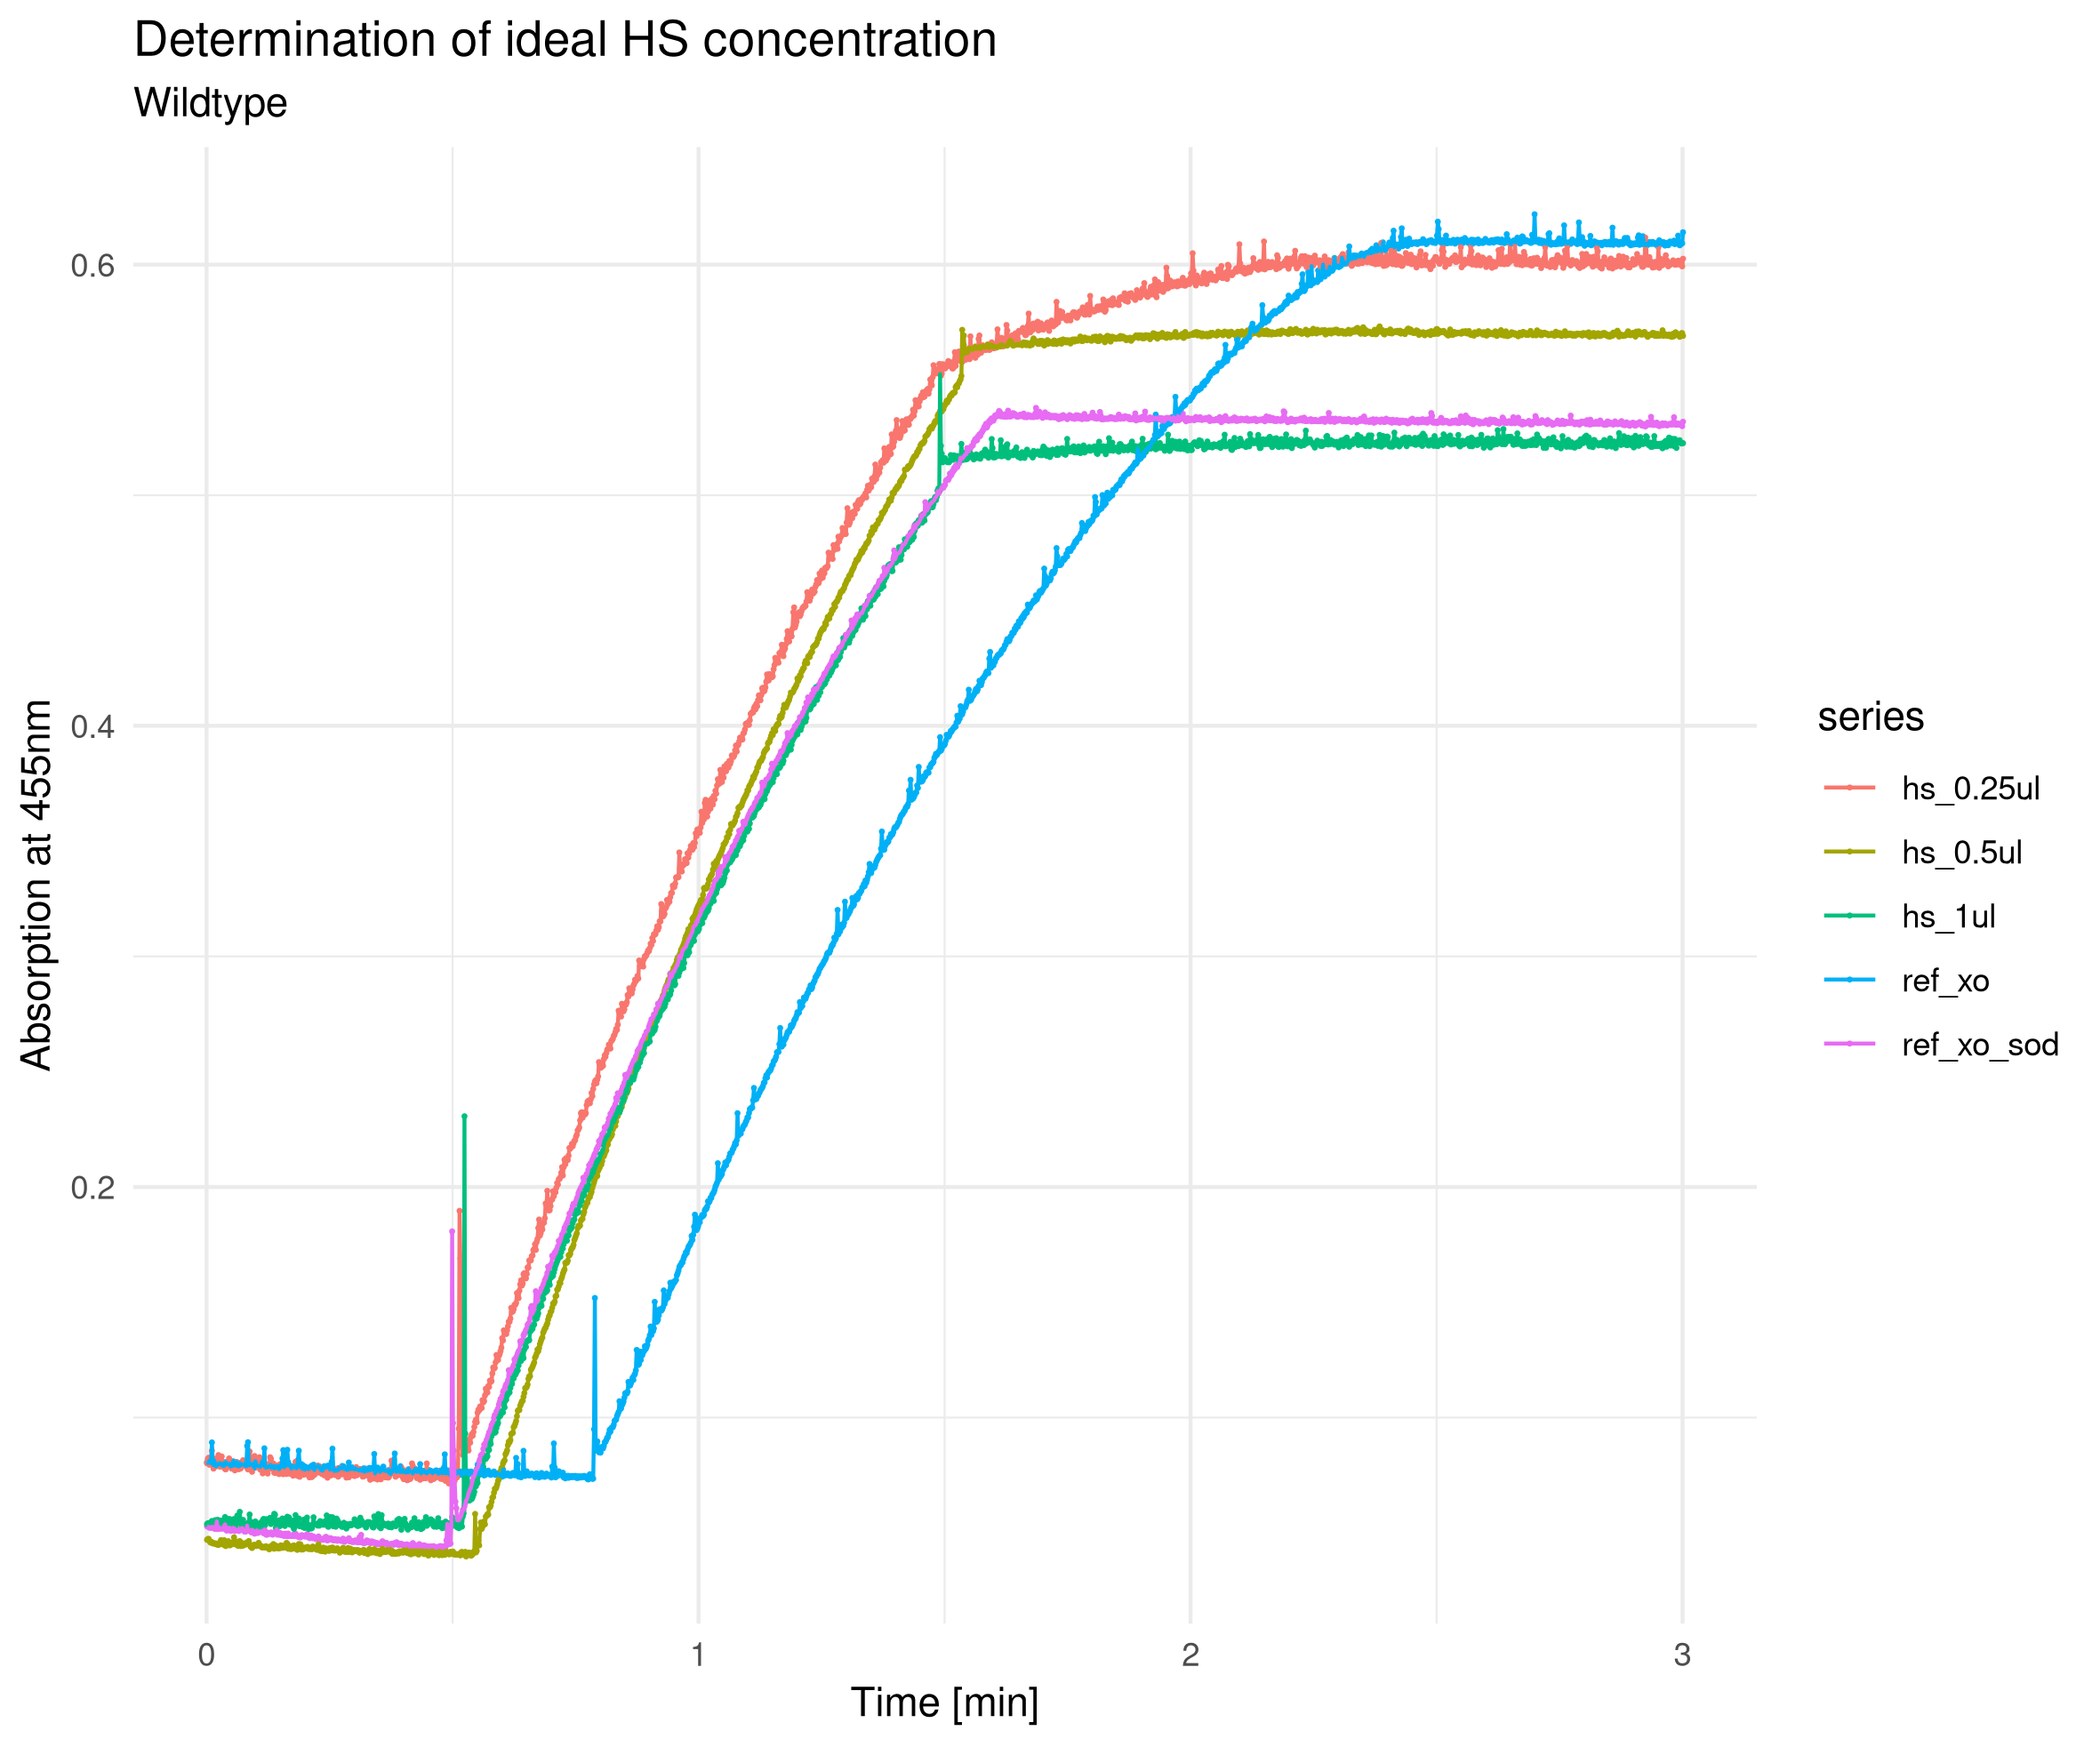
\includegraphics[width=\textwidth]{img/activity_wt_hs.png}
	\caption{HS wildtype}
	\label{fig:activity_wt_hs}
    \end{subfigure}
    \caption{Determination of sufficient HS concentration}
    \label{fig:activity_hs}
\end{figure}

\begin{figure}
    \centering
    \begin{subfigure}{0.75\textwidth}
	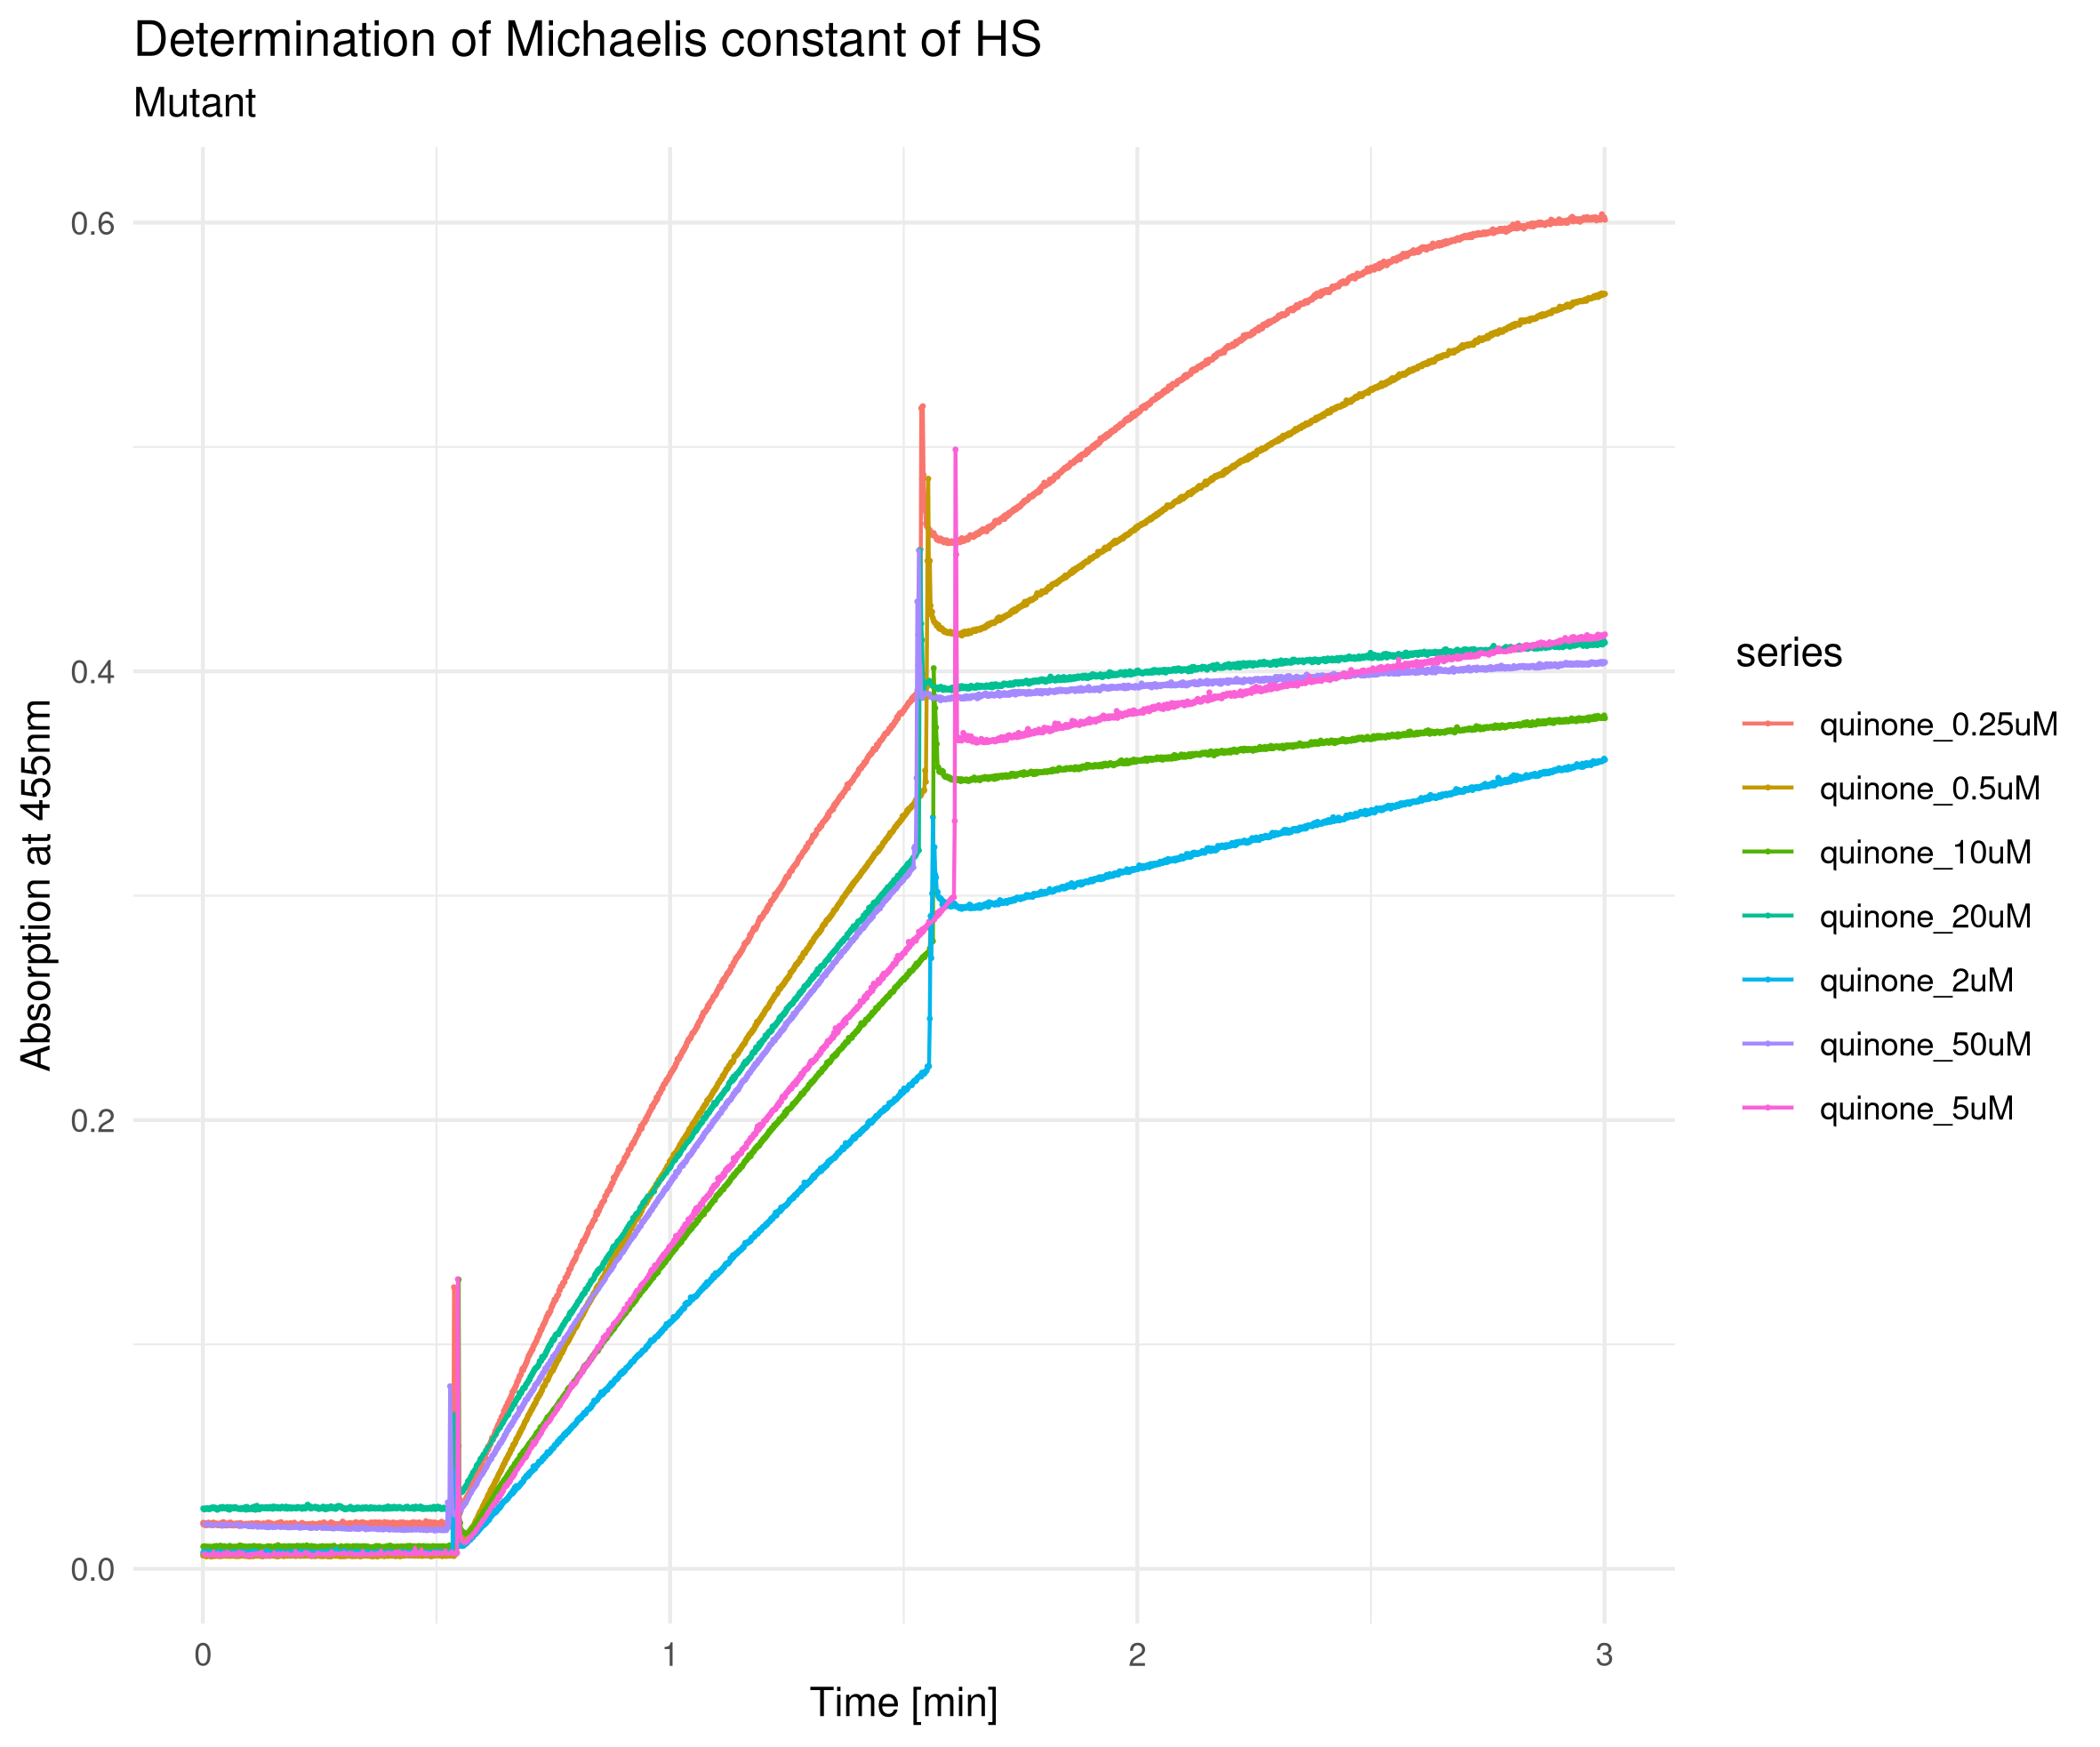
\includegraphics[width=\textwidth]{img/activity_mut_quinone.png}
	\caption{HS mutant}
	\label{fig:activity_mut_quinone}
    \end{subfigure}

    \begin{subfigure}{0.75\textwidth}
	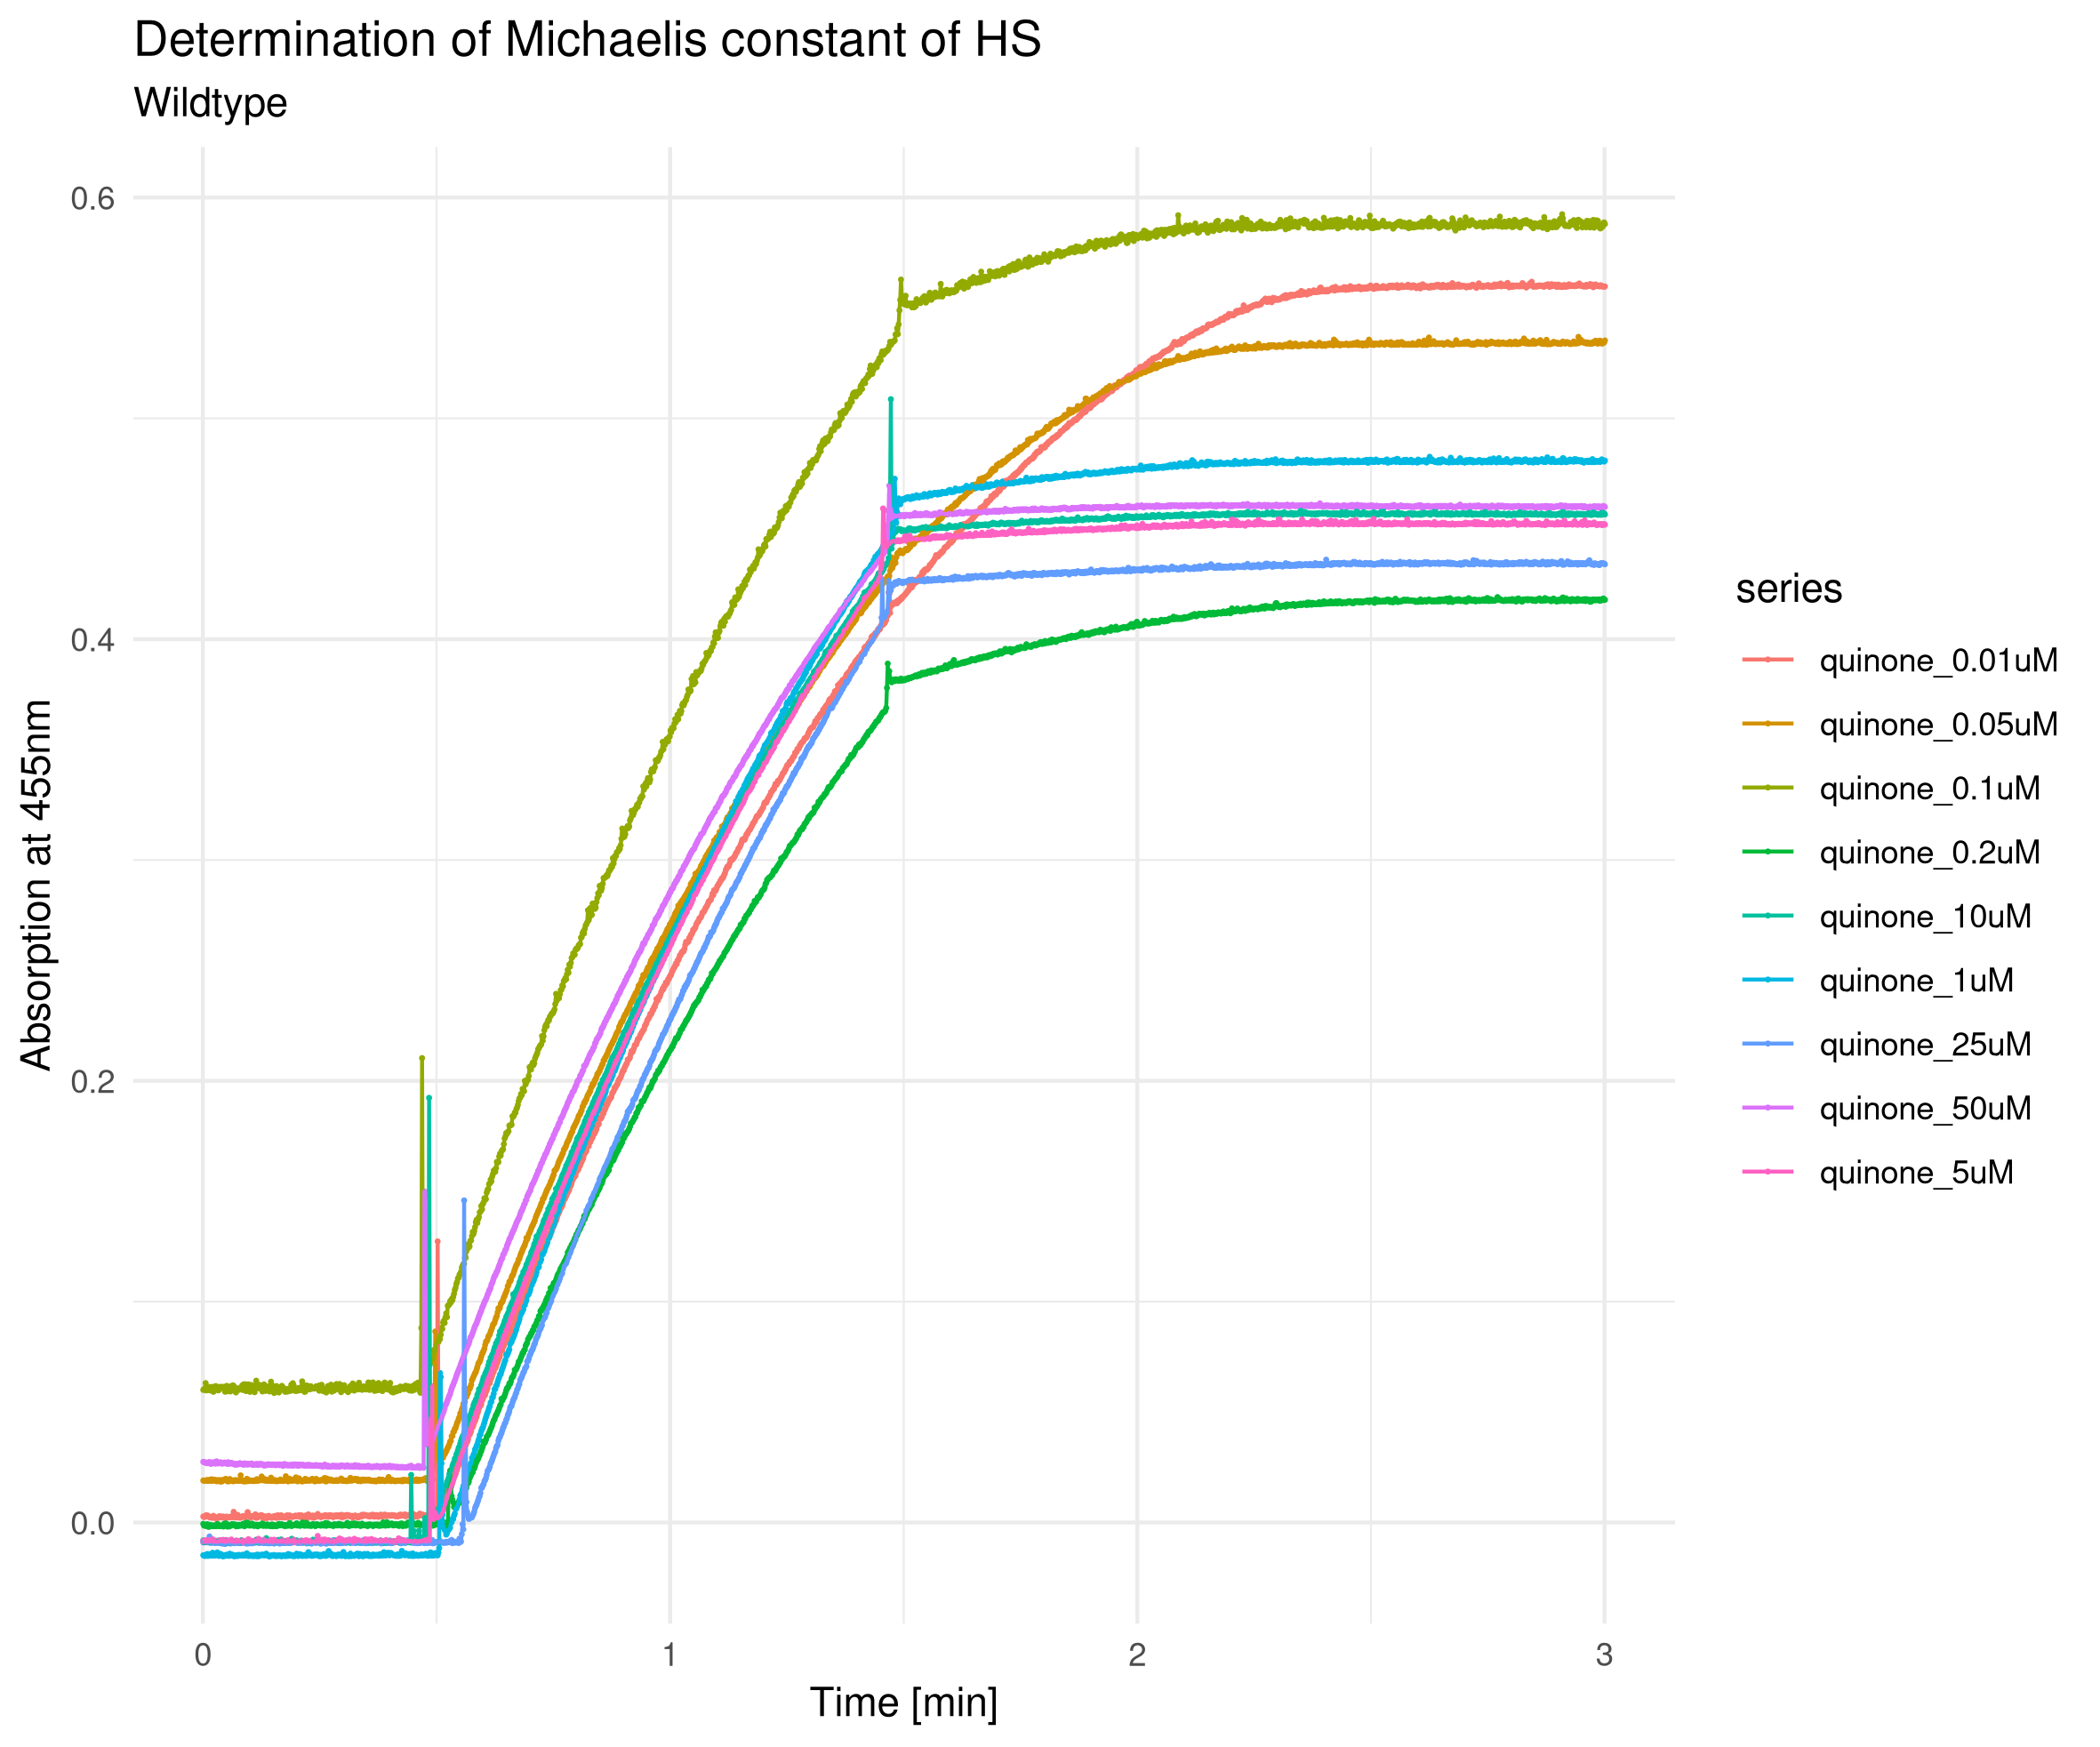
\includegraphics[width=\textwidth]{img/activity_wt_quinone.png}
	\caption{HS wildtype}
	\label{fig:activity_wt_quinone}
    \end{subfigure}
    \caption{Determination of activity depending on Quinone concentration}
    \label{fig:activity_quinone}
\end{figure}

\begin{figure}
    \centering
    \begin{subfigure}{0.45\textwidth}
	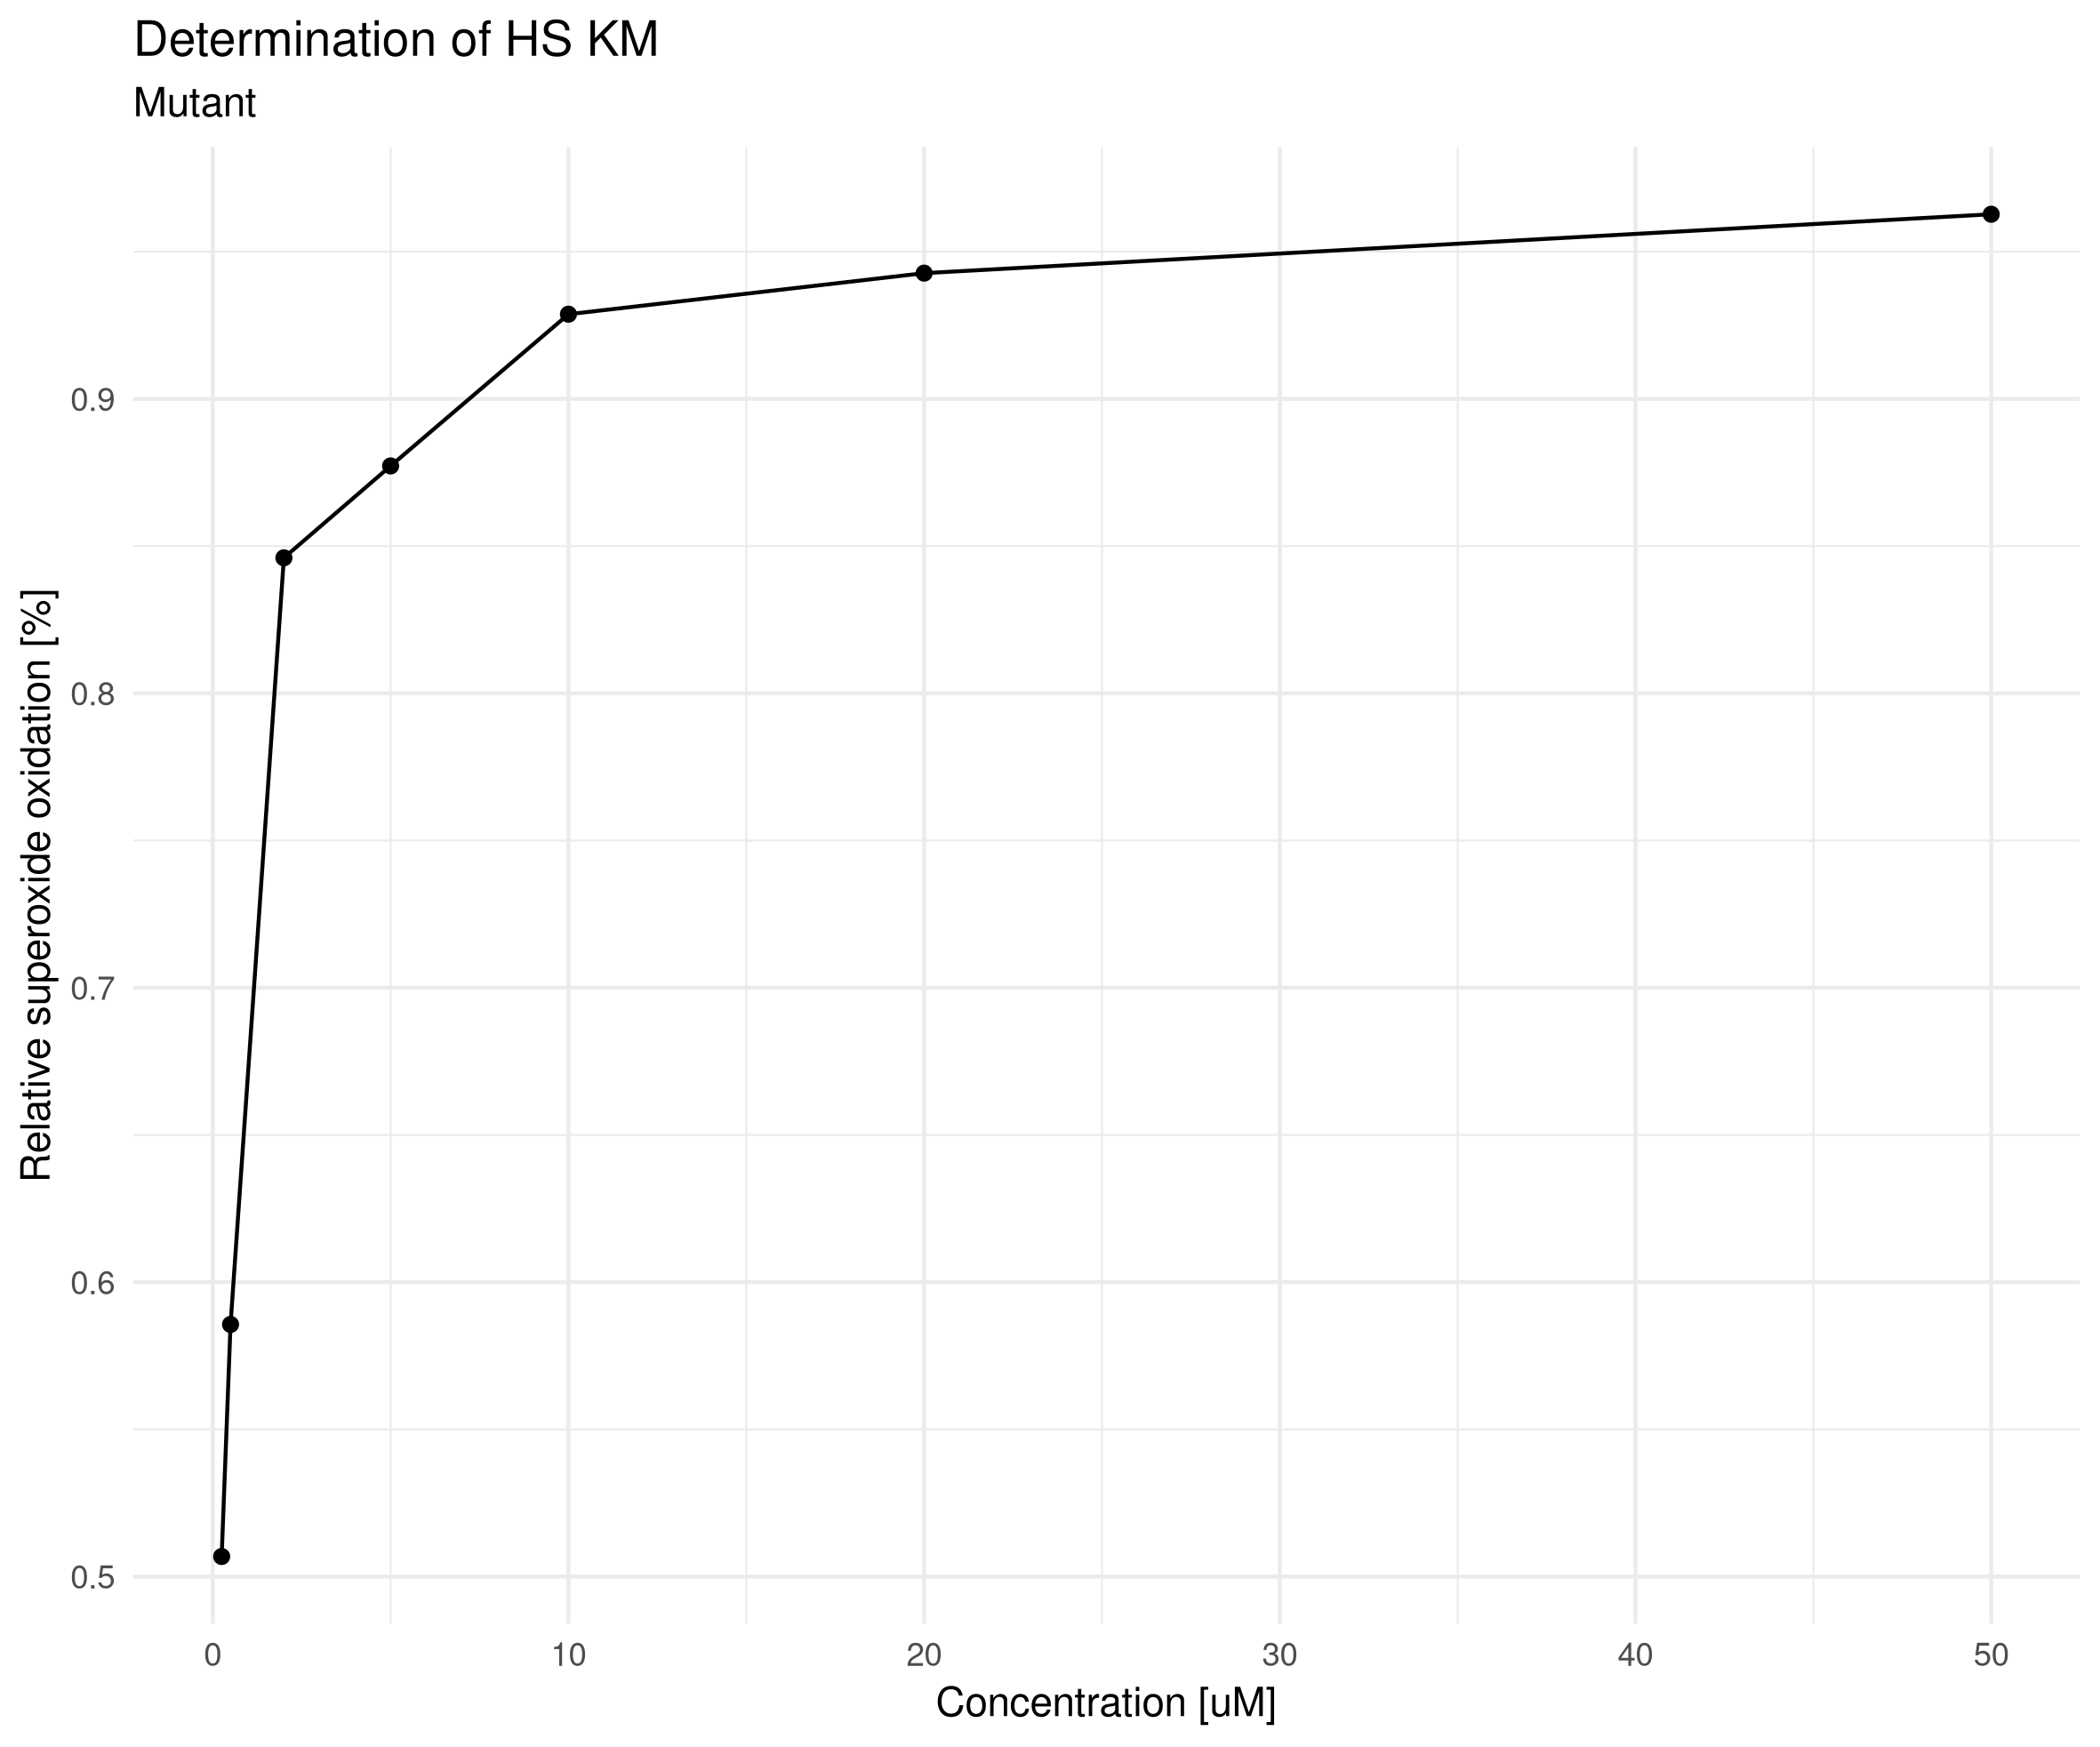
\includegraphics[width=\textwidth]{img/activity_mut_km.png}
	\caption{HS mutant}
	\label{fig:activity_mut_km}
    \end{subfigure}
    ~
    \begin{subfigure}{0.45\textwidth}
	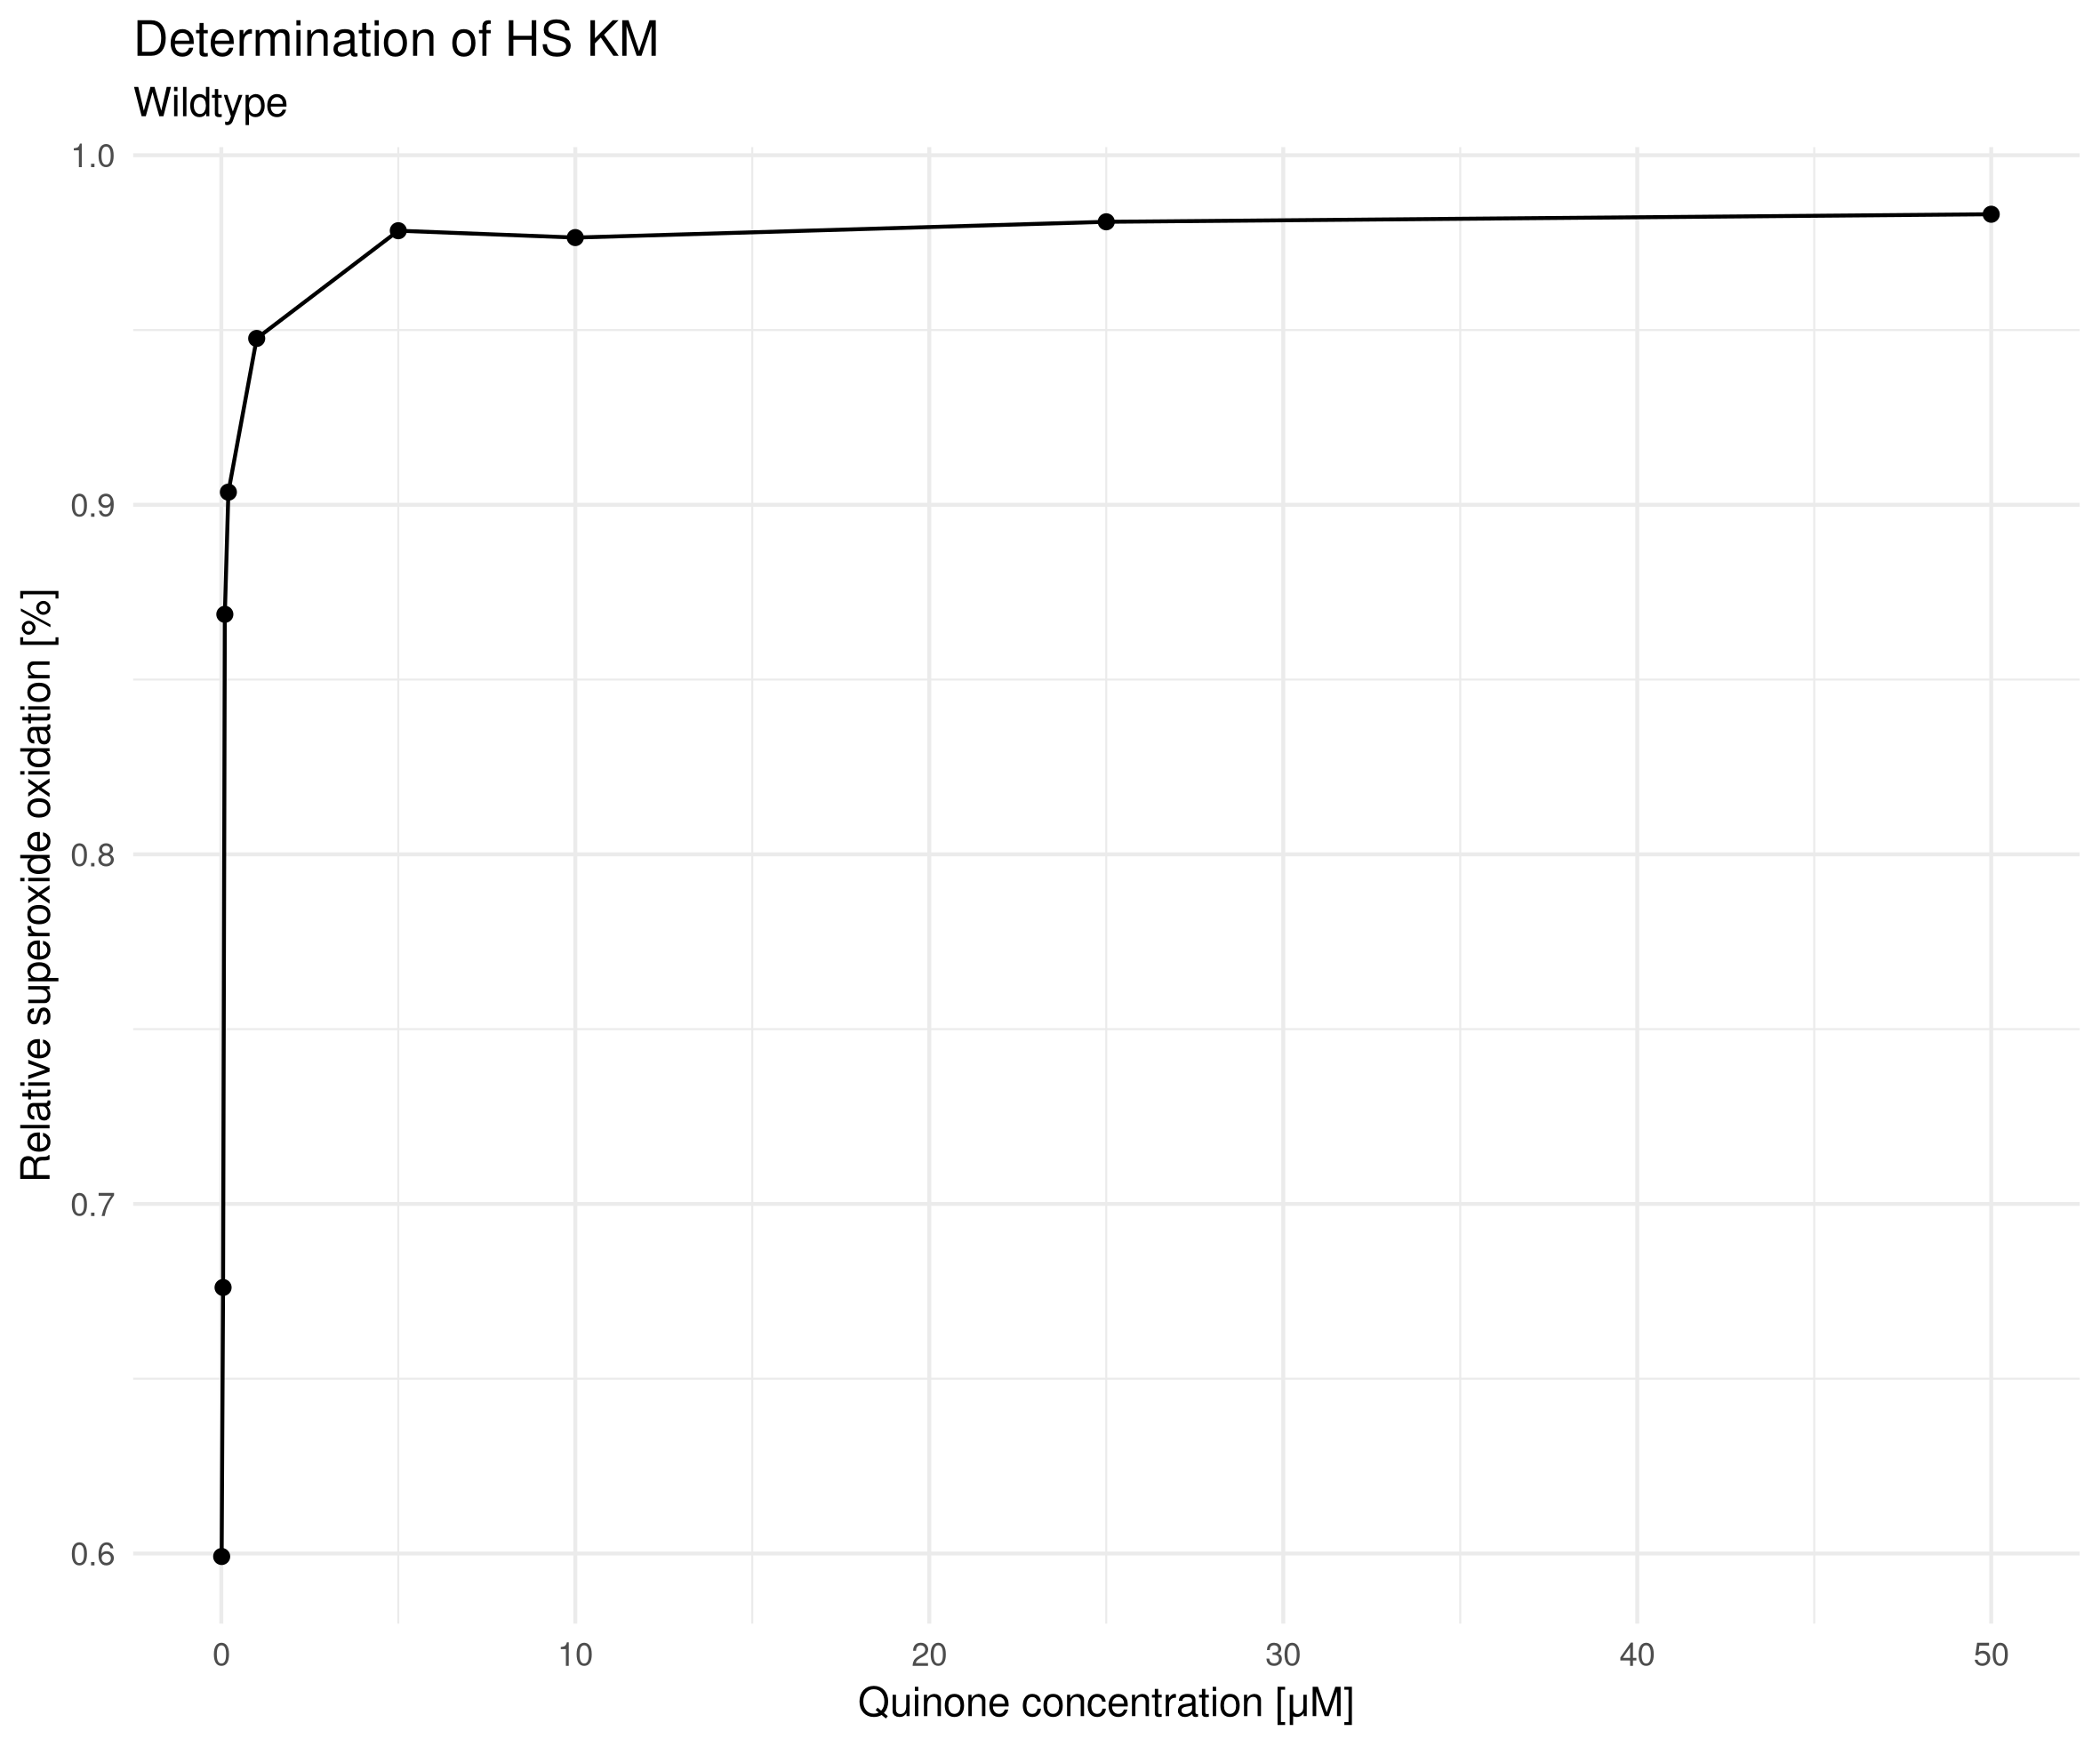
\includegraphics[width=\textwidth]{img/activity_wt_km.png}
	\caption{HS wildtype}
	\label{fig:activity_wt_km}
    \end{subfigure}
    \caption{Determination of relative superoxide oxidation per quinone concentration}
    \label{fig:activity_km}
\end{figure}

\begin{figure}
    \centering
    \begin{subfigure}{0.45\textwidth}
	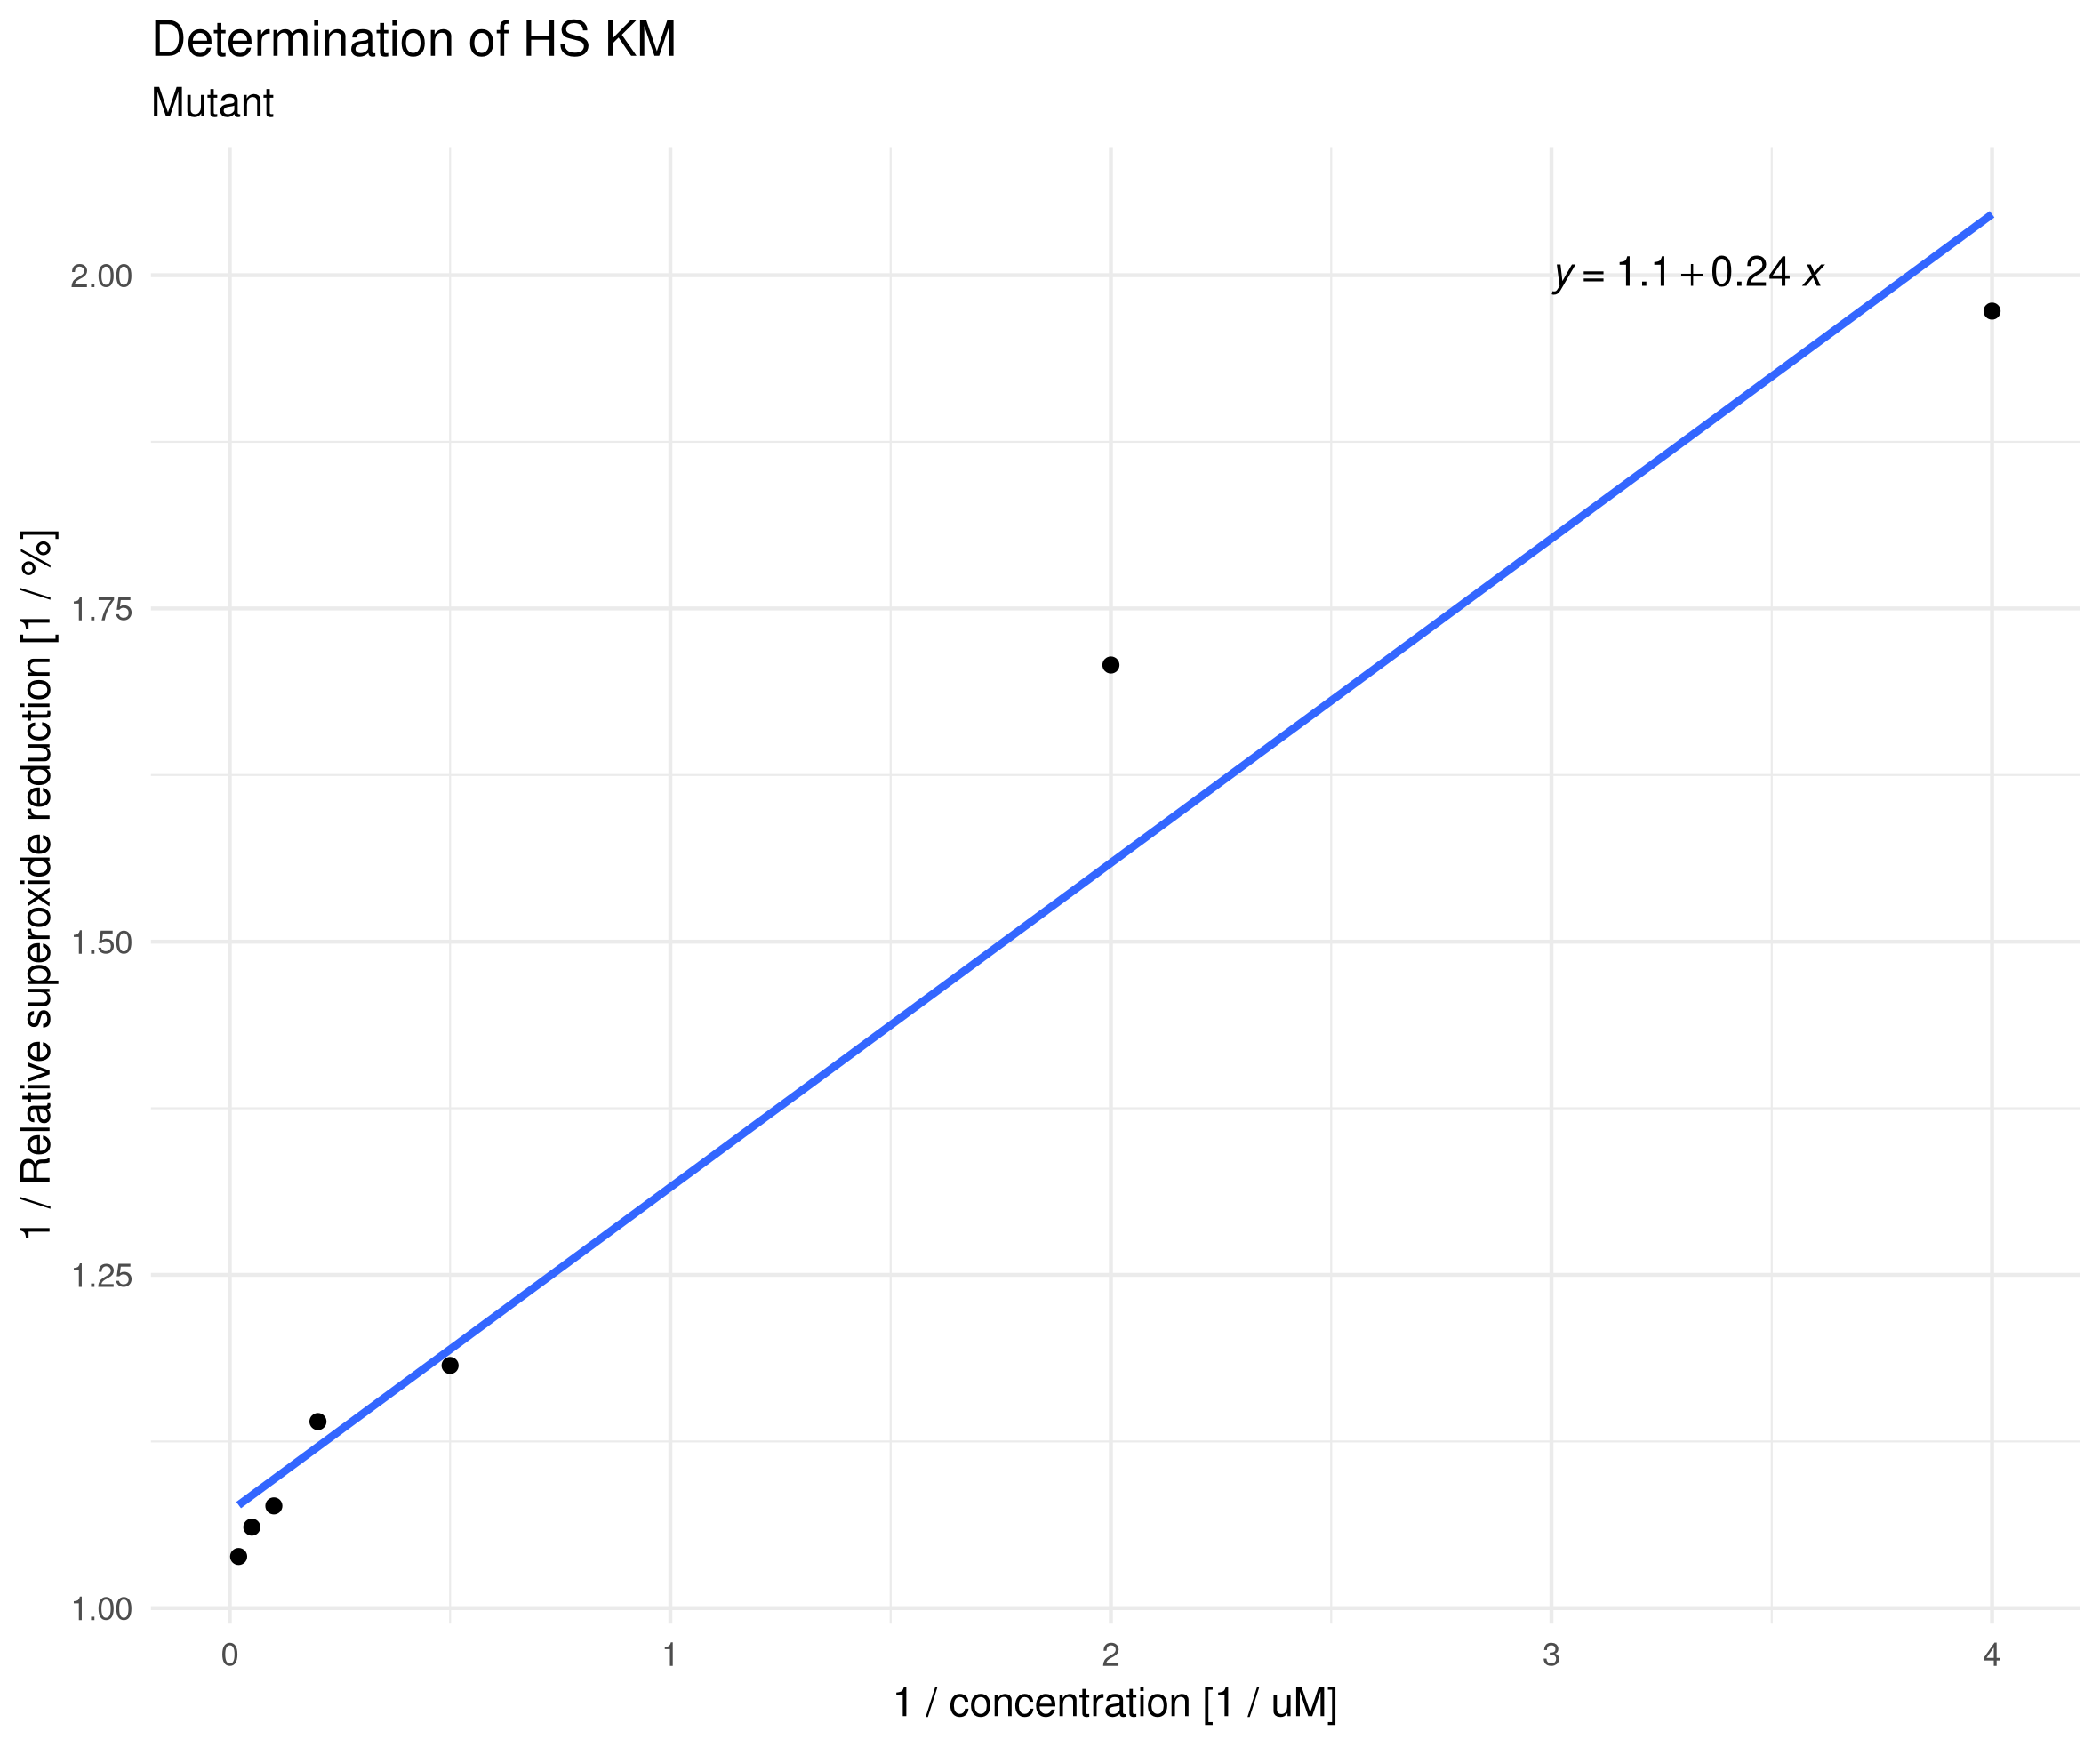
\includegraphics[width=\textwidth]{img/activity_mut_km_lb.png}
	\caption{HS mutant}
	\label{fig:activity_mut_km_lb}
    \end{subfigure}
    ~
    \begin{subfigure}{0.45\textwidth}
	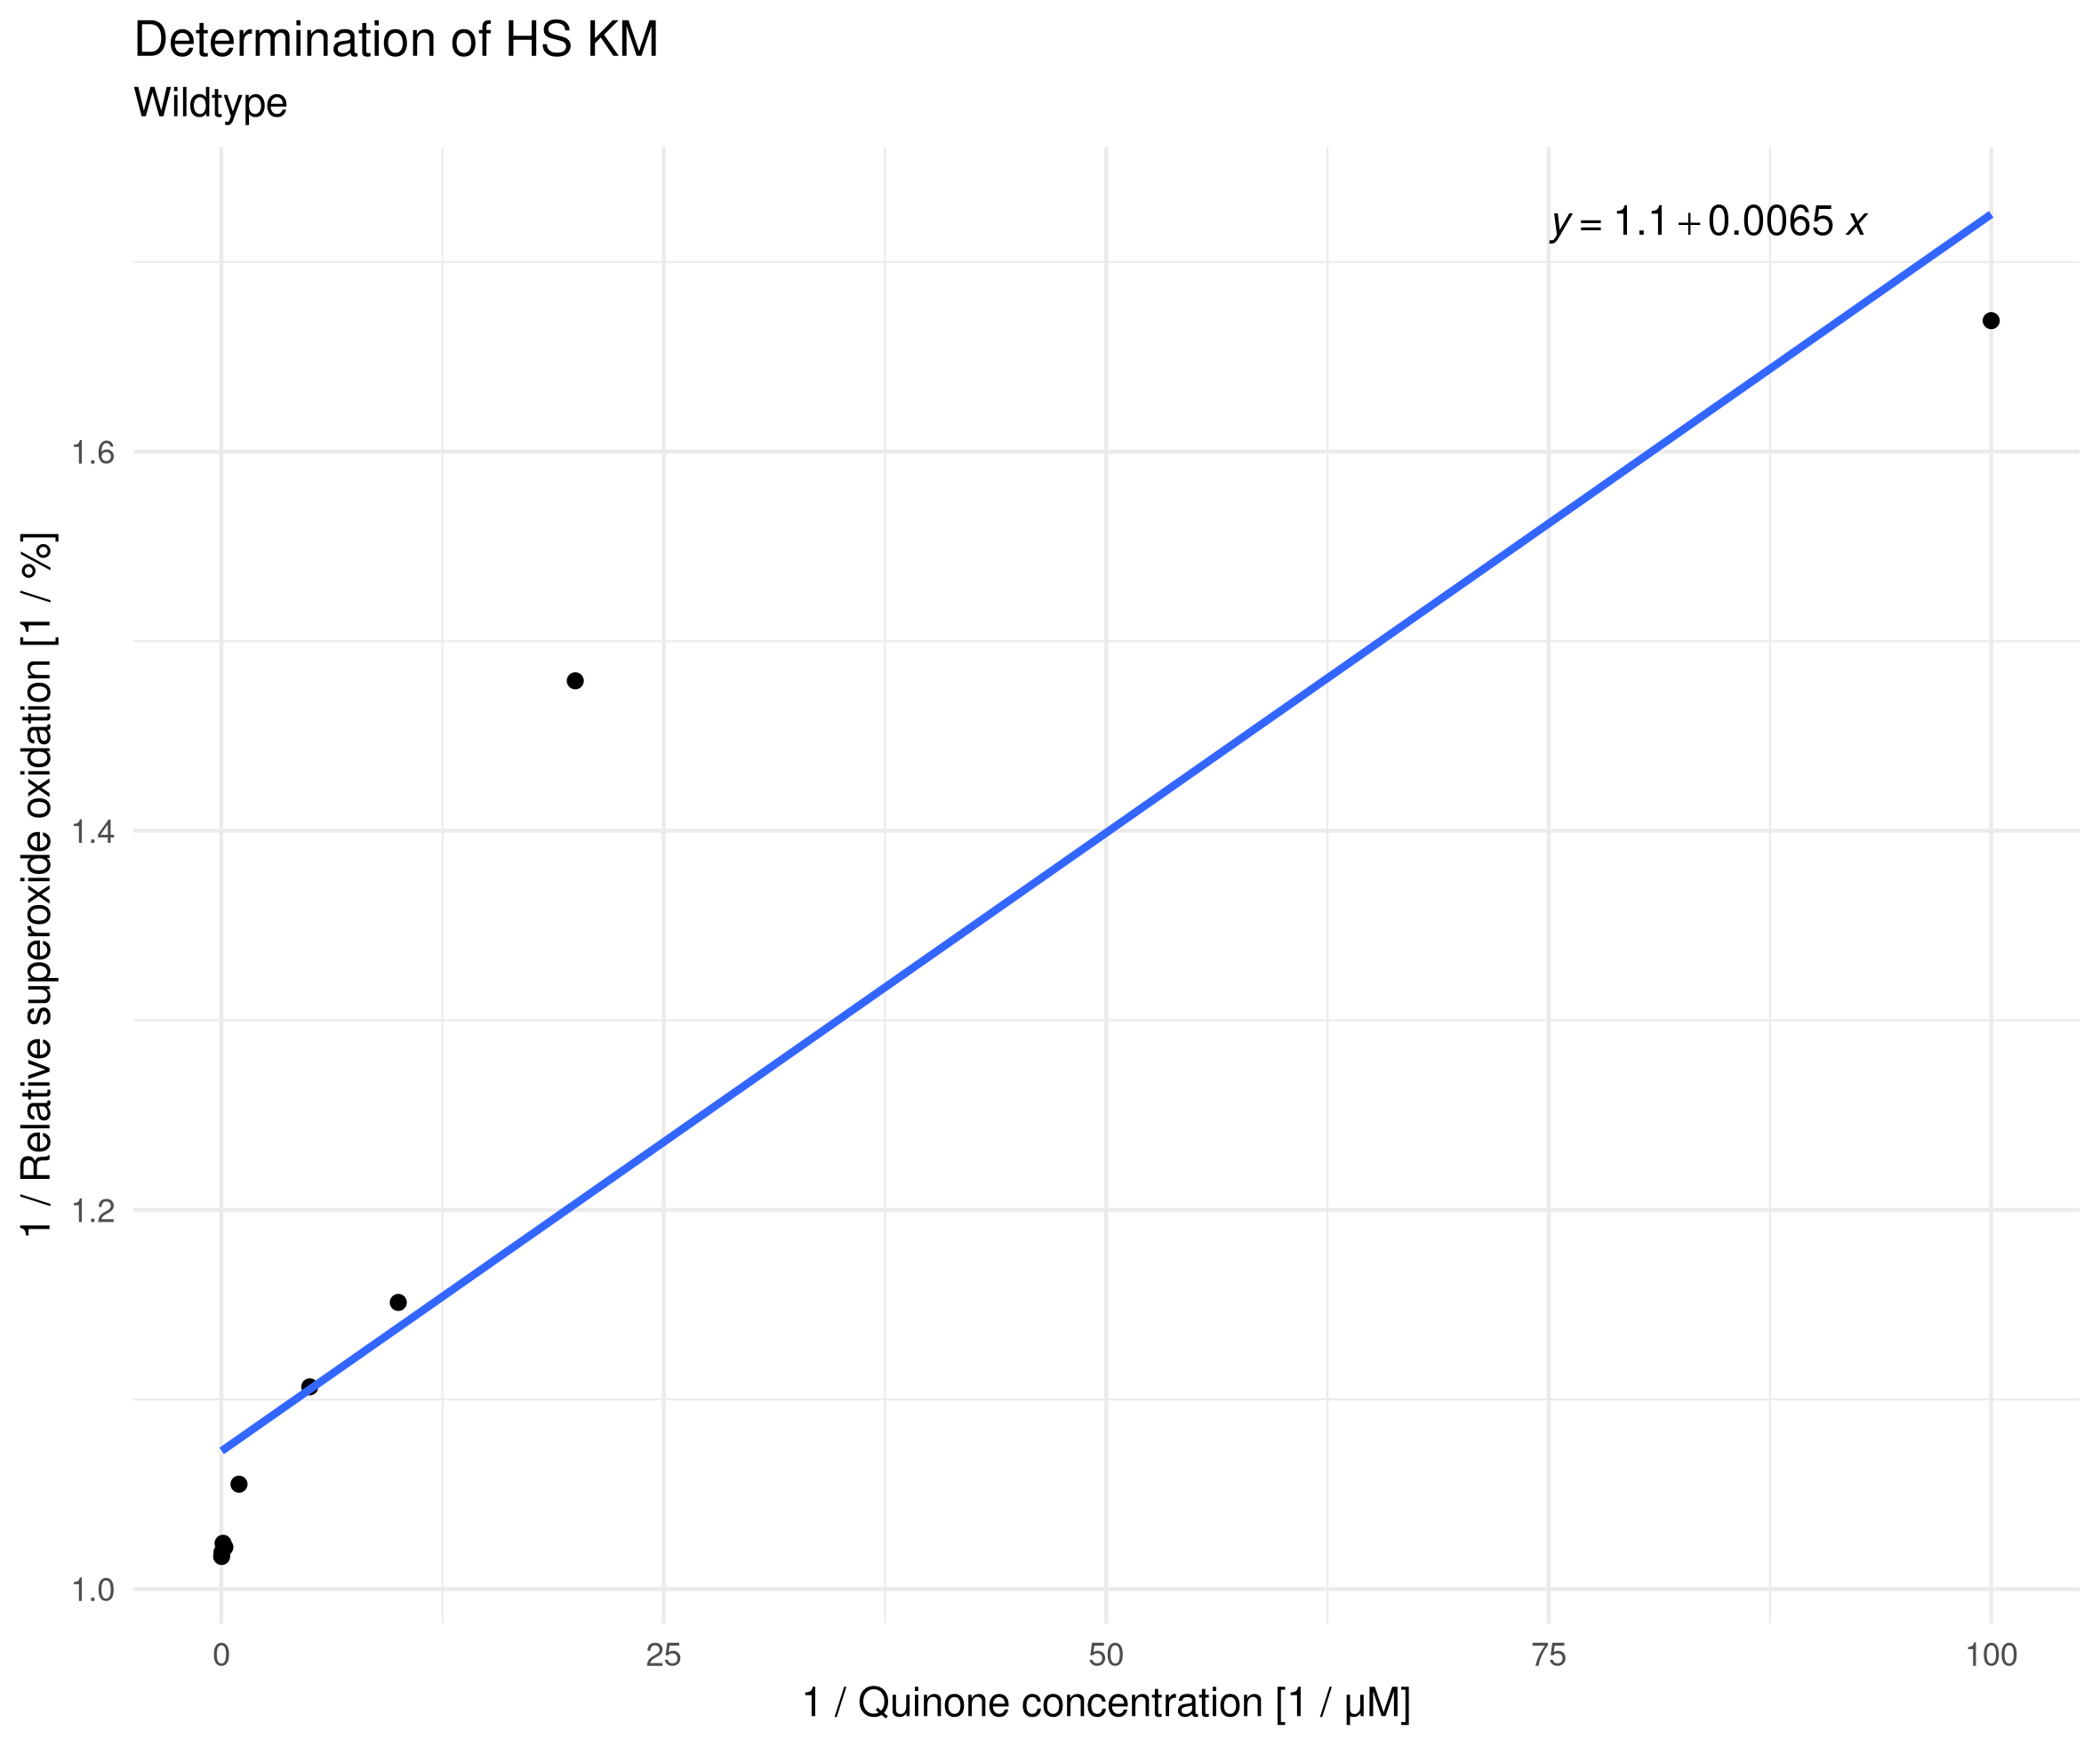
\includegraphics[width=\textwidth]{img/activity_wt_km_lb.png}
	\caption{HS wildtype}
	\label{fig:activity_wt_km_lb}
    \end{subfigure}
    \caption{Determination of $K_m$}
    \label{fig:activity_km_lb}
\end{figure}

\chapter{Discussion}

\section{Size exclusion chromatography}

In all three SEC graphs there are peaks next to the main one, which imply that
there were impurities within the column. Impurities which are in later
fractions than SOO took longer to pass through the columns, hence contain
molecules which are smaller than SOO. Similarly impurities which are in earlier
fractions are larger than SOO.

This step allowed to further purify the protein, allowing to filter not only on
the affinity to His-tagged nickel beads as was done before, but in addition to
filter based on the size of molecules.

\section{Protein concentration determination}

The determined concentration of the wild type and mutant is comparable, while
the one of dsRed is significantly bigger. This matches the observation that the
dsRed pellet at the beginning of purification was heavier.

\section{SDS PAGE}

\subsection{Purification}

\subsubsection{Flowthrough}

In all three samples the flowthrough contained many compounds of different
size. These were all compounds which were unable to bind to the column, hence
which did not have a His tag.

\subsubsection{Wash}

The wash samples of the wildtype and mutant did not contain a lot, whereas the
one of dsRed contained a variety of compounds found both in the flowthrough, as
well as in later stages. This might imply that the column used for dsRed had
been loaded above capacity.

\subsubsection{Wash \SI{5}{\milli\Molar}}

The \SI{5}{\milli\Molar} His wash allowed to wash out everything which was able
to weakly bind to the column, without washing out the strongly bound SOO.
Comparing the bands with the bands from later purification steps which are
known to be SOO imply that a bit of SOO was washed out in this step.

\subsubsection{Before ÄKTA}

The before ÄKTA lanes were the result of the elution of the column with
\SI{100}{\milli\Molar} His. The big bands are likely the HS. Of interest is
that, for the wildtype and mutant the big bands are around \SI{17}{\kilo\Da},
while for dsRed they are between \SIrange{43}{55}{\kilo\Da}. This implies that
the dsRed HS forms trimers, whose size would be around \SI{51}{\kilo\Da}. As
this behaviour is only seen in small amounts for the wildtype, and barely for
the mutant, dsRed itself seems to promote formation of these trimers.

To a lesser extent there are bands around \SI{34}{\kilo\Da} visible in all
three lanes, implying that all variants of HS form dimers to some extent.

\subsubsection{After ÄKTA}
The after ÄKTA lanes show that, while certain impurities were removed as in the
case of the mutant or dsRed, or at least had their concentration lowered as in
the case of the wildtype, a bit of HS was lost as well for all three proteins.

\subsection{dsRed cleavage}

Comparing the before ÄKTA lane with the before loading lane, between which the
sample was incubated with TEV protease, shows the lane around \SI{51}{\kilo\Da}
disappeared, while the one around \SI{17}{\kilo\Da}, known to be the band of
the HS wild type, got stronger. This implies that cleavage was successful.

There is an additional band visible slightly below \SI{26}{\kilo\Da}, which can
be identifies as the TEV protease by comparing it with the lane where only TEV
protease was loaded.

The flowthrough only contains HS at \SI{17}{\kilo\Da}, which is expected as
both the TEV protease as well as dsRed are His-tagged, so will have stayed
bound to the column. Similarly the elution then contained bands which
correspond with the TEV protease.

\section{Fluorescence measurements}

\subsection{Membrane extraction}

In the first step where cells were cracked open in the maximator there were
barely any losses of proteins. This is to be expected as care was taken to not
discard any proteins left inside the maximator.

The ultracentrifugation step seems to have already lead to significant losses
though, hinting that either there were still some membranes left in solution
rather than in the pellet, or parts of the pellet had been lost. One approach
to try and lower these losses would be to centrifuge for longer, or potentially
multiple times.

\subsection{Affinity chromatrography}

As the fluoroescence of the flowthrough was comparably high it would seem that
too much protein was loaded onto the column, so some was unable to bind. This
also matches the observation for the corresponding sample in the SDS-PAGE gel
mentioned above. This lead to some losses of proteins.

The wash step with plain buffer did not seem to cause any significant loss of
proteins, while the one with \SI{5}{\milli\Molar} Hist did cause the early
elution of some proteins. This might be hard to avoid as some His-tagged
protein is guaranteed to bind to the wash buffer.

The fluorescence of the elution, when compared to the fluoroescence of the last
step of the membrane extraction, then shows that not too much protein was lost
during the affinity chromatography.

\subsection{Reverse IMAC}

The fluorescence of the elution and flowthrough stages confirms what was
already seen in the SDS-PAGE gel - the majority of the fluorescent dsRed was
in the elution, so bound to the column. Only a small part was in the
flowthrough, which might eg be dsRed which was washed out by the
\SI{5}{\milli\Molar} His wash buffer.

\section{Relative enzyme reduction}

For both quinol and superoxide the negative control confirms that the change in
absorbance was caused by the reduction of HS, and not by something unrelated.
In either case are the relative reductions of the wild type and mutant
comparable, implying that the mutation does not have a direct effect on the
equilibrium.

\subsection{Superoxide as substrate}

The relative reduction of samples where SOD was added clearly shows that SOD is
able to quench the reduction of HS, by quickly removing superoxide from the
system.

The data shows that the relative reduction of solubilized enzymes is
significantly higher than those of reconstituted enzymes. This might imply that
superoxide is unable to enter liposomes, such that in the case of liposomes it
cannot reduce those HS enzymes whose active site is within the liposome. Such
an observation was also made in the one of the referenced papers \cite{soo}.
Under the assumption that this holds we can estimate, by comparing the relative
reduction of reconstituted and solubilized enzymes, that in liposomes about
half the enzymes have one orientation, while the other half has another.

\subsection{Quinol as substrate}

The reduction of the reconstituted HS is close to the theoretical maximum of
\SI{50}{\percent}, as only one of the two Hems can be reduced by quinol
addition. Of interest is that the relative reduction of solubilized HS is
significantly lower than that of the reconstituted. This might either be an
experimental error which further experiments could clarify, or quinol has an
easier time binding to reconstituted enzymes over solubilized ones.

\section{Fluorescence measurements before and after cleavage}

\subsection{Solubilized dsRed}

The measurements with solubilized dsRed served to show that the method works.
There is clear fluorescence in the first measurement, which can be quenched
significantly by adding copper, and restored by adding the chelating agent
EDTA.

\subsection{Uncleaved liposomes}

The exact same behaviour can be observed with uncleaved liposomes. As
fluorescence is heavily quenched upon adding a lot of copper one can assume
that the vast majority, if not all, dsRed is oriented towards the outside of
the liposome. The remaining bit of fluorescence might either be dsRed which is
oriented towards the inside of the liposome, or a lacking amount of copper
added. This can also be seen in the second measurement with a higher volume of
liposomes, where not all fluoroescence could be quenched.

\subsection{Cleaved liposomes}

With cleaved liposomes there was a significantly lower initial fluorescence
compared with uncleaved ones. This confirms that cleavage itself was a success.
As this fluorescence can be quenched with copper, however, there must be
uncleaved dsRed left oriented towards the outside of the liposomes, as copper
cannot enter those. This implies that cleavage was not complete, and a longer
incubation or higher concentration of TEV protease would be needed.

\section{Activity measurement}

The equal to within rounding limits $v_{\text{max}}$ imply that the mutation
does not impede the maximum speed of the enzyme in case of an overwhelming
substrate concentration. The $K_m$ values however, which differ by two orders
of magnitude, imply that the mutation significantly lowers the affinity of the
enzyme for quinone, lowering its speed in a system with low substrate
concentration.
